\nomenclature[A]{CRC}{Cyclic Redundancy Check}
\nomenclature[A]{TOF}{Time of Flight}
\nomenclature[A]{DS-TWR}{Double Sided Two Way Ranging}
\nomenclature[A]{API}{Application Programming Interface}
\nomenclature[A]{SPI}{Serial Peripheral Interface Bus}
\nomenclature[A]{IRQ}{Interrupt Request}
\nomenclature[A]{GPIO}{General Purpose Input/Output Pin}
In this chapter, we describe in detail the design (Section 5.1), key design choices (Section 5.2), and the implementation details (Section 5.3) of the Test Platform for evaluation and analysis of UWB (TP-UWB).

\section{Test Platform Design}
The test platform as shown in Figure \ref{fig:phasesOfTestPlatform} consists of five phases:
\begin{figure}[h!]
	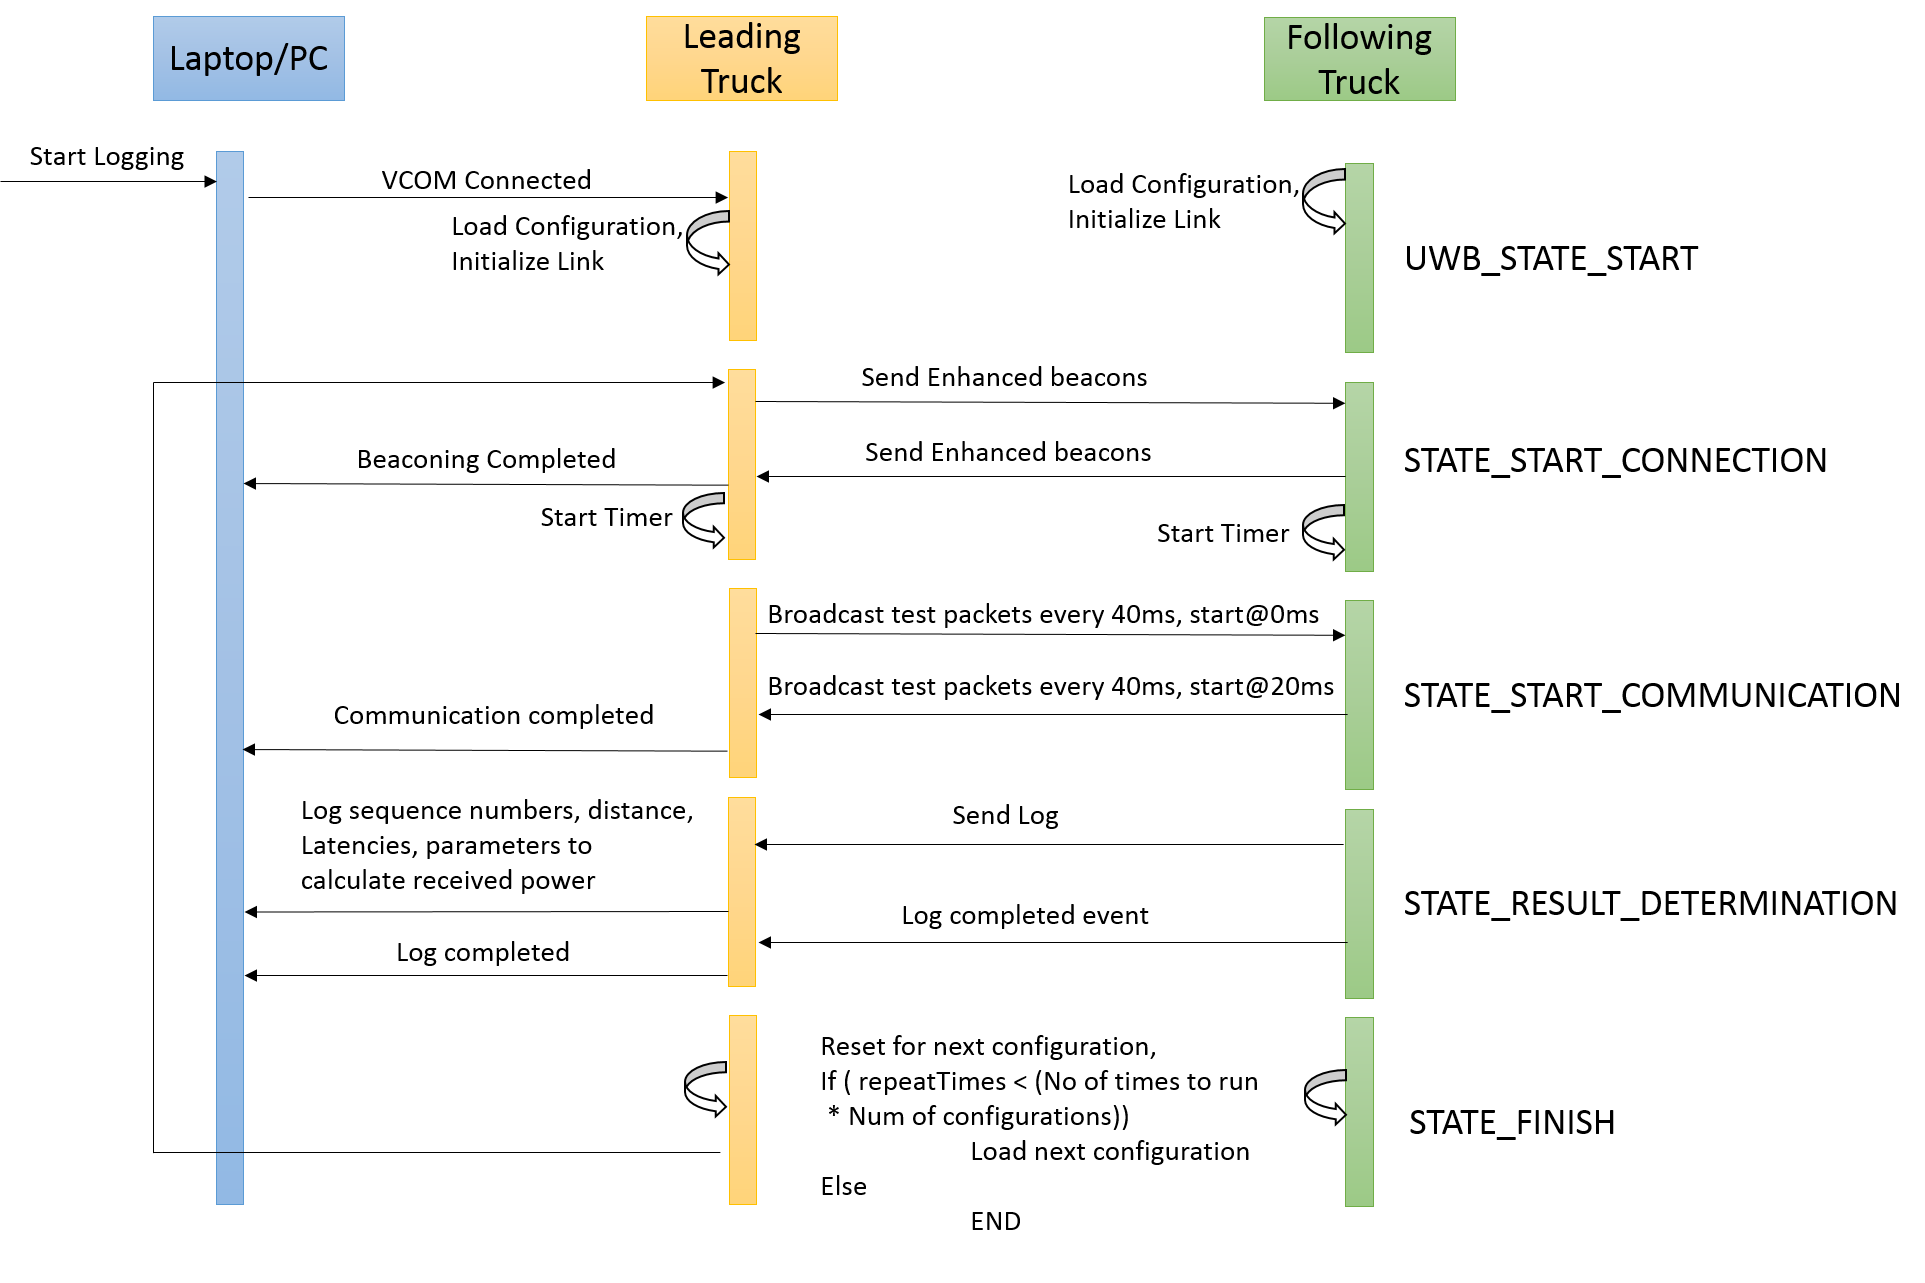
\includegraphics[width=1\textwidth,keepaspectratio]{figures/PhasesofTestPlatform}
	\centering
	\caption{Phases of test platform}
	\label{fig:phasesOfTestPlatform}    
\end{figure}
\begin{enumerate}
    \item \textbf{UWB\_STATE\_START}: In this phase, the leading truck will be waiting for the VCOM connected event from the laptop/PC to start execution. Once it receives this event, the first configuration is loaded, and the link is initialized. The following truck does not wait for the VCOM connected event and starts execution on power-up wherein the first configuration is loaded, and the link is initialized. In link initialization, we set the MAC address of the node, configure event counters, set the receiver to infinite timeout, set preamble detect to infinite timeout, enable frame filtering only to accept acknowledgment, data and beacon frames destined to that particular node. Also, we enable interrupts for frame sent, frame received with good CRC, receiver PHY header error, receiver CRC error, receiver sync loss error, frame wait timeout, preamble detect timeout, SFD timeout and frame rejected. Moreover, we set the pointer to the TX callback function that gets executed after the transfer of a packet and set the pointer to the RX callback function that gets executed after the reception of a packet.
    
    \item \textbf{STATE\_START\_CONNECTION}: In this phase, the following truck will be waiting infinitely for the first beacon. The leading truck will transmit a beacon every 10 ms starting at 0 ms instant and wait for the reception of a beacon from the following truck until the next transmission. In each beacon, it transmits the remaining number of beacons it requires to go to next state. Similarly, the following truck sends a beacon (indicating the required remaining number of beacons) every 5 ms and waits for the reception of a beacon from the leading truck until next transmission. Once a defined number of beacons are received sequentially, the leading truck and the following truck go into the next state respectively.  
    
    \item \textbf{STATE\_START\_COMMUNICATION}: In this phase, the leading truck broadcasts test messages every 40 ms starting at 0 ms time instant and the following truck broadcasts text messages every 40 ms starting at 20 ms time instant. We synchronize on the reception of the first packet from the leading truck to the following truck. The following truck stores the log information (sequence numbers, message latency, packet latency, distance and values for calculation of received power level) of the test packet received from the leading truck.
    
    \item \textbf{STATE\_RESULT\_DETERMINATION}: In this phase, the following truck sends the stored log information of the received test packets to the leading truck. The leading truck on receiving this log information, sends it serially to the laptop, along with its log information of the received test packets from the following truck.
    
    \item \textbf{STATE\_FINISH}: During this phase, we reset for execution of the next configuration, if (repeatTimes \textless (No of times to run * Number of configurations)), we load the next configuration and go to the STATE\_START\_CONNECTION phase, else the test is stopped.
    
\end{enumerate}

%Phases of Test Platform
%Ranging
%State Machine of Leading Truck
%State Machine of Following Truck
%For each phase, process flow
%What happens during Transmission
%What happens during Reception etc...


\section{Important Design Choices}
Below we list the key design choices of the test platform:
\begin{enumerate}
    \item Suitable ranging method: We have three different ways, the pros and cons of each method are provided in Table \ref{table:DesignChoiceRanging}. We choose Double Sided Two Way Ranging (DS-TWR) as the method for implementing ranging attributed to the facts that the number of packets required for ranging is small when the application is considered for a large number of following trucks, reply times can be asymmetric, and error in calculated TOF is minimized. Also, the processor on LPCXpresso4337 can easily handle multiplication and division operations in a short duration of time.
   \begin{table}
       \centering
       \begin{longtable}{@{\extracolsep{\fill}}| p{2.55cm}  | p{4.8cm} | p{5cm} | p{5cm} |@{}}
           \hline
           \centering {\textbf{Design Choice}} &\centering {\textbf{Pros}   }                                                                                                                                                                                                   & \centering {\textbf{Cons}}                                                                                                                                                                                                                                                                                                                                                                                                                                                                                                     \\ \vspace{-3mm}\hline
           Single Sided Two way Ranging  & \vspace{-7mm} \begin{itemize}[leftmargin=*]
               \item Only one message exchange required which saves time \& power (within approx. 40 ms + delta time, the ranging value can be determined).\end{itemize}   & \vspace{-7mm} \begin{itemize}[leftmargin=*]
               \item Time of Flight (TOF) estimate error increases as Treply increases (turn around time) and as clock offset increases. 
               \item If tight tolerance clocks are used, Treply is short \& communication range is relatively short then it might be worthy of examination.   \end{itemize}\\                                                                                                                                                                                        \hline
           Double Sided Two way Ranging          &  \vspace{-7mm} \begin{itemize}[leftmargin=*] \item Reply times need not be the same. \item Error in calculated TOF is minimized. \item In case of platooning, the number of packets required to determine the range = N+2 (N=Number of following trucks). \end{itemize}& \vspace{-7mm} \begin{itemize}[leftmargin=*] \item Requires multiplication and division operations. \item Requires 4 messages to determine the range \item Within approx. 80 ms + delta time, the ranging value can be determined.  \end{itemize}                                                                                                      \\ \hline
           Symmetric Double-Sided Two way Ranging  & \vspace{-7mm} \begin{itemize}[leftmargin=*] \item Requires only simple math operations to derive a result. \end{itemize}                                                                                                                                                                                & \vspace{-7mm} \begin{itemize}[leftmargin=*] \item Does not seem suitable for platooning when the number of trucks in the platoon is increased as the number of packets required for ranging = 3N (N= Number of following trucks). \item Reply times must be the same - difficult to achieve. \item Error induced is proportional to difference between the reply times. \item The ranging exchange is longer than necessary because all reply times must be as long as the longest reply time. \item Increase in latency. \end{itemize} \\ \hline
           \caption{Design Choice - Ranging}
           \label{table:DesignChoiceRanging}
       \end{longtable}
   \end{table}
    \item Compliance to standards or non-compliance to standards: This question arises due to the additional 39 bytes (maximum value) of MAC header for each packet. The pros and cons of these two options are indicated in the Table \ref{table:ComplianceStandardsvsNonCompliance}. We choose to comply to the IEEE 802.15.4 standard so as to support interoperability, and hence break messages (\textgreater 127 bytes) into several 127 byte packets. 
    % Please add the following required packages to your document preamble:
    % \usepackage{graphicx}
   % Please add the following required packages to your document preamble:
   % \usepackage{graphicx}
   \begin{table}
       \centering
       \begin{longtable}{| p{2.55cm}  | p{4.8cm} | p{5cm} | p{5cm} |}
           \hline
           \centering {\textbf{Design Choice}} &\centering {\textbf{Pros}   }                                                                                                                                                                          & \centering {\textbf{Cons}}                                                                                                                                                                                                                                                                                                                                                                                                                                                                                                                                                                                                                                                               \\ \vspace{-3mm}\hline
           Compliance to Standards     &  \vspace{-7mm} \begin{itemize}[leftmargin=*] \item Interoperability: Ability of devices to work together relies on products and services complying with standards. \item Reliability \& Safety: More dependable. \item Foundation for new features \item Business benefits: Market access, awareness, etc.\end{itemize} & 
           \vspace{-7mm} \begin{itemize}[leftmargin=*] \item Additional latency during communication. \item Increase in coding complexity as messages (\textgreater 127 bytes) need to be broken down into several 127 byte packets\end{itemize} \\ \hline
           Non Compliance to Standards & \vspace{-7mm} \begin{itemize}[leftmargin=*] \item Decrease in latency during communication. \item Decrease in coding complexity.\end{itemize}                                                                                                                                                                              & \vspace{-7mm} \begin{itemize}[leftmargin=*] \item Incompatibility with other equipment. \item Restricted to one manufacturer or supplier\end{itemize}                                                  \\ \hline
       \end{longtable}
       \caption{Compliance to Standards vs Non Compliance}
       \label{table:ComplianceStandardsvsNonCompliance}
   \end{table}
    
    \item Choice of data rate: The pros and cons for all the available three data rates are provided in the table \ref{table:prosconsdatarate}. We make use of all the three data rates in different measurement plans attributed to their respective advantages.
   % Please add the following required packages to your document preamble:
   % \usepackage{graphicx}
   \begin{table}
       \centering
       \begin{longtable}{| p{2.55cm}  | p{4.8cm} | p{5cm} | p{5cm} |}
           \hline
           \centering {\textbf{Data Rate Parameter} }& \centering {\textbf{Pros}     }                                                                                                                                                                                               & \centering {\textbf{Cons}      }                                                                                                          \\ \vspace{-3mm}\hline
           110 Kbps                     & \vspace{-7mm} \begin{itemize}[leftmargin=*] \item Range of signal increases. \item Ideal for better ranging results and high multipath environments.\end{itemize}                                                                       & \vspace{-7mm} \begin{itemize}[leftmargin=*] \item Very high latency (13.5424 ms). \end{itemize}                                                                                            \\ \hline
           850 Kbps                     & \vspace{-7mm} \begin{itemize}[leftmargin=*] \item Latency better than that of 110 kbps (2.2430 ms). \item Ranging accuracy better than that of 6.8 Mbps. \end{itemize}                                                                     & \vspace{-7mm} \begin{itemize}[leftmargin=*] \item Latency more than that of 6.8 Mbps. \item Ranging accuracy less than that of 110 Kbps.\end{itemize} \\ \hline
           6.8 Mbps                     & \vspace{-7mm} \begin{itemize}[leftmargin=*] \item Low latency (0.4404 ms). \item Data rate similar to that of 802.11p. \item Shortened Tx and Rx times, better battery \& appropriate for burst interference environments.\end{itemize} & \vspace{-7mm} \begin{itemize}[leftmargin=*] \item Ranging accuracy will be reduced, \item Range/distance reduces\end{itemize}                        \\ \hline
       \end{longtable}
       \caption{Pros/Cons - Data Rate}
       \label{table:prosconsdatarate}
   \end{table}
    
    \item Choice of Preamble Length and SFD or Non-standard SFD:  
    \begin{itemize}
        \item \textbf{Shorter preamble length}: Reduces transmission and reception time.
        \item \textbf{Longer preamble length}: Guarantees higher security, improves range and ranging accuracy.
        \item \textbf{Non-standard SFD sequence}: More robust than IEEE 802.15.4 standard, improved performance and improved ranging accuracy because of more accurate time stamps.
        \item \textbf{Standard SFD sequence}: If we use non-standard SFD, it will be impossible to inter-work with a device expecting a standard SFD sequence.
    \end{itemize}    
    From the above facts, instead of choosing a single preamble length or Standard SFD or non-standard SFD, we use them as a sweep parameter to determine the influence of these factors on the performance of UWB.   
    \item The test platform consists of two application binaries which will be flashed into the respective devices (leading truck and the following truck). One application implements the functions of the leading truck and will be flashed to the leading truck and other implements the functions of the following truck and will be flashed into the following truck.
    \item We send data communication packets from the leading truck to the following truck and vice-versa every 40 ms according to the typical platooning application requirement.
    \item We log the values onto the laptop/computer only at the end of configuration execution because printing the logs serially during communication causes deviation from the desired schedule when the COM port is busy. Hence we store the required values until the end of configuration execution.
    \item Limited by the logging information that can be stored in RAM, we send 250 messages when we have three or four packets per message and 500 messages when we have two or one packet per message.
    \item There exist state transitions in the leading truck and the following truck. We make use of the timeout mechanism in both leading truck and the following truck to come out of a phase if it does not receive within the maximum time window. For example, in the communication state, both nodes transmit messages at their respective time instants irrespective of whether a message is received or not and move into the next state as designed.
    \item We operate in two settings: reliable and test settings. We make use of 110 Kbps data rate in the reliable settings. We are in reliable settings during the STATE RESULT DETERMINATION. We use test settings during the STATE START COMMUNICATION. The test settings are based on the current test case.
    \item There are four types of messages exchanged between the nodes namely: MSG ID TEST DATA, MSG ID COMMUNICATION RESULT, ACK, BEACON in states STATE START COMMUNICATION, STATE RESULT DETERMINATION, STATE RESULT DETERMINATION, STATE START CONNECTION respectively.
    \item The following truck synchronizes on the first communication packet received in the STATE START COMMUNICATION. We do not use beacons to synchronize every message considering the additional packet that needs to be transmitted. The additional packet for every message plays a significant role considering the latency and LDC requirements of the system, and operation of the platooning application.
    
\end{enumerate}
\section{Architecture}
The system is designed to operate as a UWB subsystem in the platooning system as shown in Figure \ref{fig:integrationOfUWBToExistingSystem} wherein UWB acts as a secondary independent back up channel.
The software overview of TP\_UWB is shown in Figure \ref{fig:softwareOverview}. We use NXP LPCXpresso4337 development board, which has a dual-core: Cortex M4 and M0 MCU. The DW1000 UWB transceiver is connected to LPCXpresso4337. TP\_UWB software is organized as two files namely application and link. The link file makes use of DecaWave device Application Programming Interface (API) to interact with the transceiver. 'DW1000' file ports the DecaWave device API to the LPCXpresso4337. The interface between LPCXpresso4337 and DW1000 is through the DecaWave device API, which internally makes use of a Serial Peripheral Interface Bus (SPI), an Interrupt Request (IRQ) and a General Purpose Input/Output pin (GPIO).
\begin{figure}[h!]
	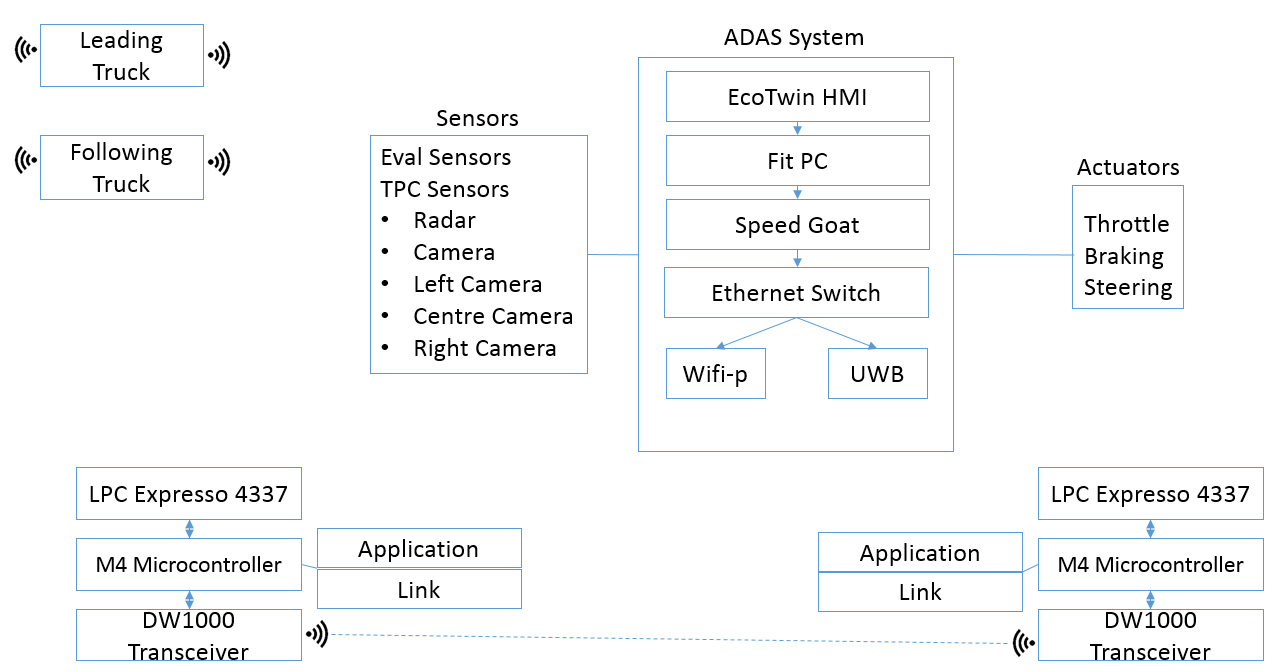
\includegraphics[width=1\textwidth]{figures/IntegrationOfUWBtoExistingSystem}
	\centering
	\caption{Wifi-p + UWB in platooning system}
	\label{fig:integrationOfUWBToExistingSystem}    
\end{figure}
\begin{figure}[h!]
    \includegraphics[width=3in]{figures/SoftwareOverview}
    \centering
    \caption{Software Overview}
    \label{fig:softwareOverview}    
\end{figure}

\section{Implementation}
Below we explain the set of actions executed in each state and the events which cause state transitions in detail.

\subsection{State Connection}
For this phase, several methods were tried. In the first method, the desired number of beacons were sent from the leading truck to the following truck, and the same number of desired beacons were sent from the following truck to the leading truck. In the latter case, the number of beacons received from the leading truck is sent in the beacons from the following truck to the leading truck. Finally, the number of beacons received from the following truck is sent in the beacons from leading to the following truck. The timeout for this phase was set to 300 ms and even on successful completion of all the above three transmissions and receptions, we wait for the elapse of this 300 ms. So that both the devices enter the next state at the same time. If the number of beacons received is more than the desired number, then the node goes to the next state, else repeat. This method did not work in all circumstances, in few special cases, the code went into infinite trials. Another method that was tried was to have 200 ms and 300 ms as respective timeout durations for leading truck and the following truck respectively. This method was also not effective.

Next method was to transmit a beacon every 10 ms from the leading truck to the following truck with the remaining number of beacons to be received to move to the next state and wait for reception of a beacon until its next transmission. Here, the following truck transmits a beacon every 5 ms to the leading truck with the remaining number of beacons to be received to move to the next state. The respective nodes were to receive a desired number of beacons to go to the next stage. This method of beaconing failed if the last beacon was received in the following truck but not in the leading truck.

The method that worked appropriately was to synchronize on the first packet that is received in the following truck from the leading truck in STATE\_COMMUNICATION. 

\subsection{State Communication}
The working of state communication phase is given in Figure \ref{fig:stateCommunication}. On entering this phase, we set a variable \emph{communicationMode} to 1 and on leaving this phase, we set it back to 0. This ensures that a part of the interrupt handler is executed only when executing in this particular phase. We set \emph{autorxreenable} to 1, so that in a case of an error during a reception, the receiver is re-enabled quickly. We set default antenna delay values for transmission and reception. 

In the case of the following truck, we set Timer2 to interrupt after 20 ms, Timer1 to interrupt every 40 ms and Timer 3 to tick every 1 $\mu$s. It is to be noted that we only set the three timers but do not enable them immediately. We enable reception for the first message. The following truck waits indefinitely for the first packet. On reception of the first packet, we enable Timer3 and Timer2. While waiting for the other packets of a message, if the Timer2 interrupt occurs then we go ahead and transmit the next message according to the schedule of every 40 ms with an offset of 20 ms from the leading truck. Even on the successful reception of the first message, we wait for Timer2 interrupt to occur. We enable Timer1, and if the messageCounter is less than or equal to \emph{NO\_OF\_MESSAGES}, then we transmit and enable reception. On the occurrence of every Timer1 interrupt, we enable Timer2 for reception timeout duration. Hence for the first instant when Timer1 is enabled, we define reception timeout for this instant using software defined timeout (Timer3). After successful/unsuccessful reception of this second message, we wait for the Timer1 interrupt to occur. It is to be noted that Timer2 is enabled in the interrupt handler of Timer1 interrupt, hence the occurrence of Timer1 interrupt indicates Timer2 is enabled for reception timeout duration. We transmit a message if messageCounter is less than or equal to \emph{NO\_OF\_MESSAGES} at this instant and enable the receiver until Timer2 interrupt. As a consequence of the successful/unsuccessful reception, we wait for Timer1 interrupt, transmit a message if messageCounter is less than or equal to \emph{NO\_OF\_MESSAGES}, and enable reception. This process continues until messageCounter is equal to the \emph{NO\_OF\_MESSAGES}.

In the case of the leading truck, we set Timer1 to interrupt every 40 ms, Timer3 to tick every 1 $\mu$s. On transmission of the first packet, we enable Timer3 and Timer1. Similar to the case of the following truck, on the occurrence of every Timer1 interrupt, we enable Timer2 for the reception timeout duration. Hence for the first instant when Timer1 is enabled, we define reception timeout for this instant using software defined timeout (Timer3). After successful/unsuccessful reception of this message, we wait for the Timer1 interrupt to occur. This process now continues very similar to that of the following truck indicated above. The test data structure data type is shown in Listing \ref{lst:testDataStructureDefinition}.

\begin{lstlisting}[caption={Test data structure definition}, label={lst:testDataStructureDefinition}, language=C]
typedef struct {
uint8 type;
uint8 timeStamp[4];
uint8 rangingMessage[32];
uint8 transferPayload[PAYLOAD_SIZE_CAN_TRANSMIT];
} msg_app_test_data;
\end{lstlisting}
\begin{figure}[h!]
    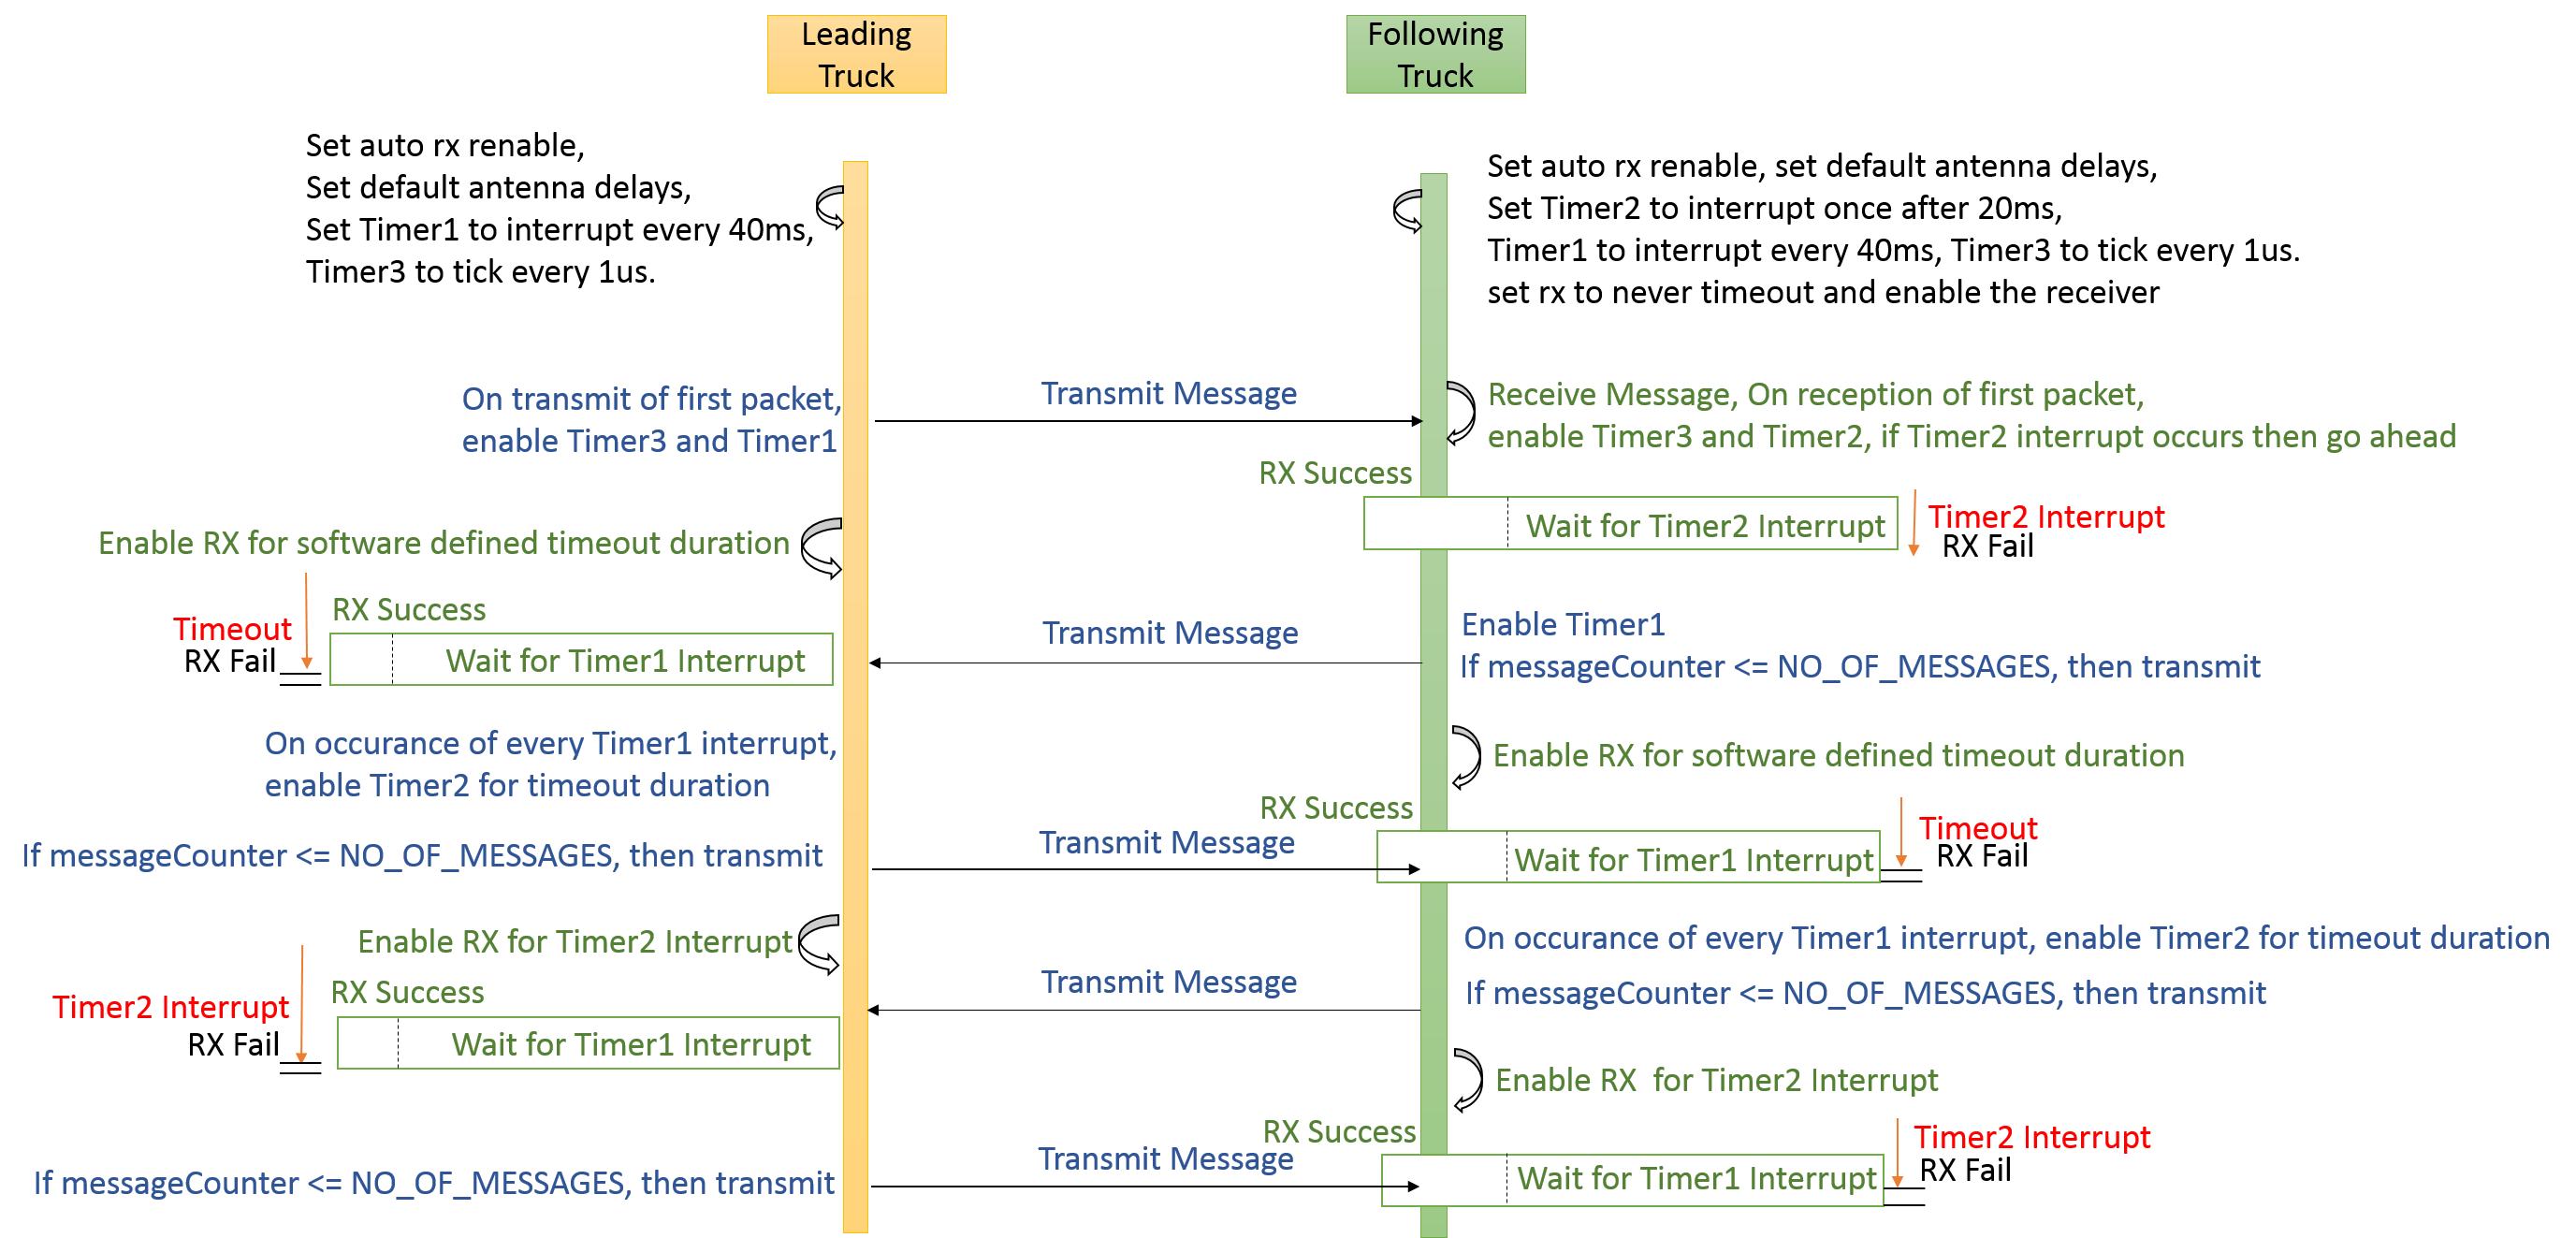
\includegraphics[width=1\textwidth]{figures/StateCommunicationPhase}
    \centering
    \caption{Process flow in State Communication}
    \label{fig:stateCommunication}    
\end{figure}
\begin{figure}[h!]
	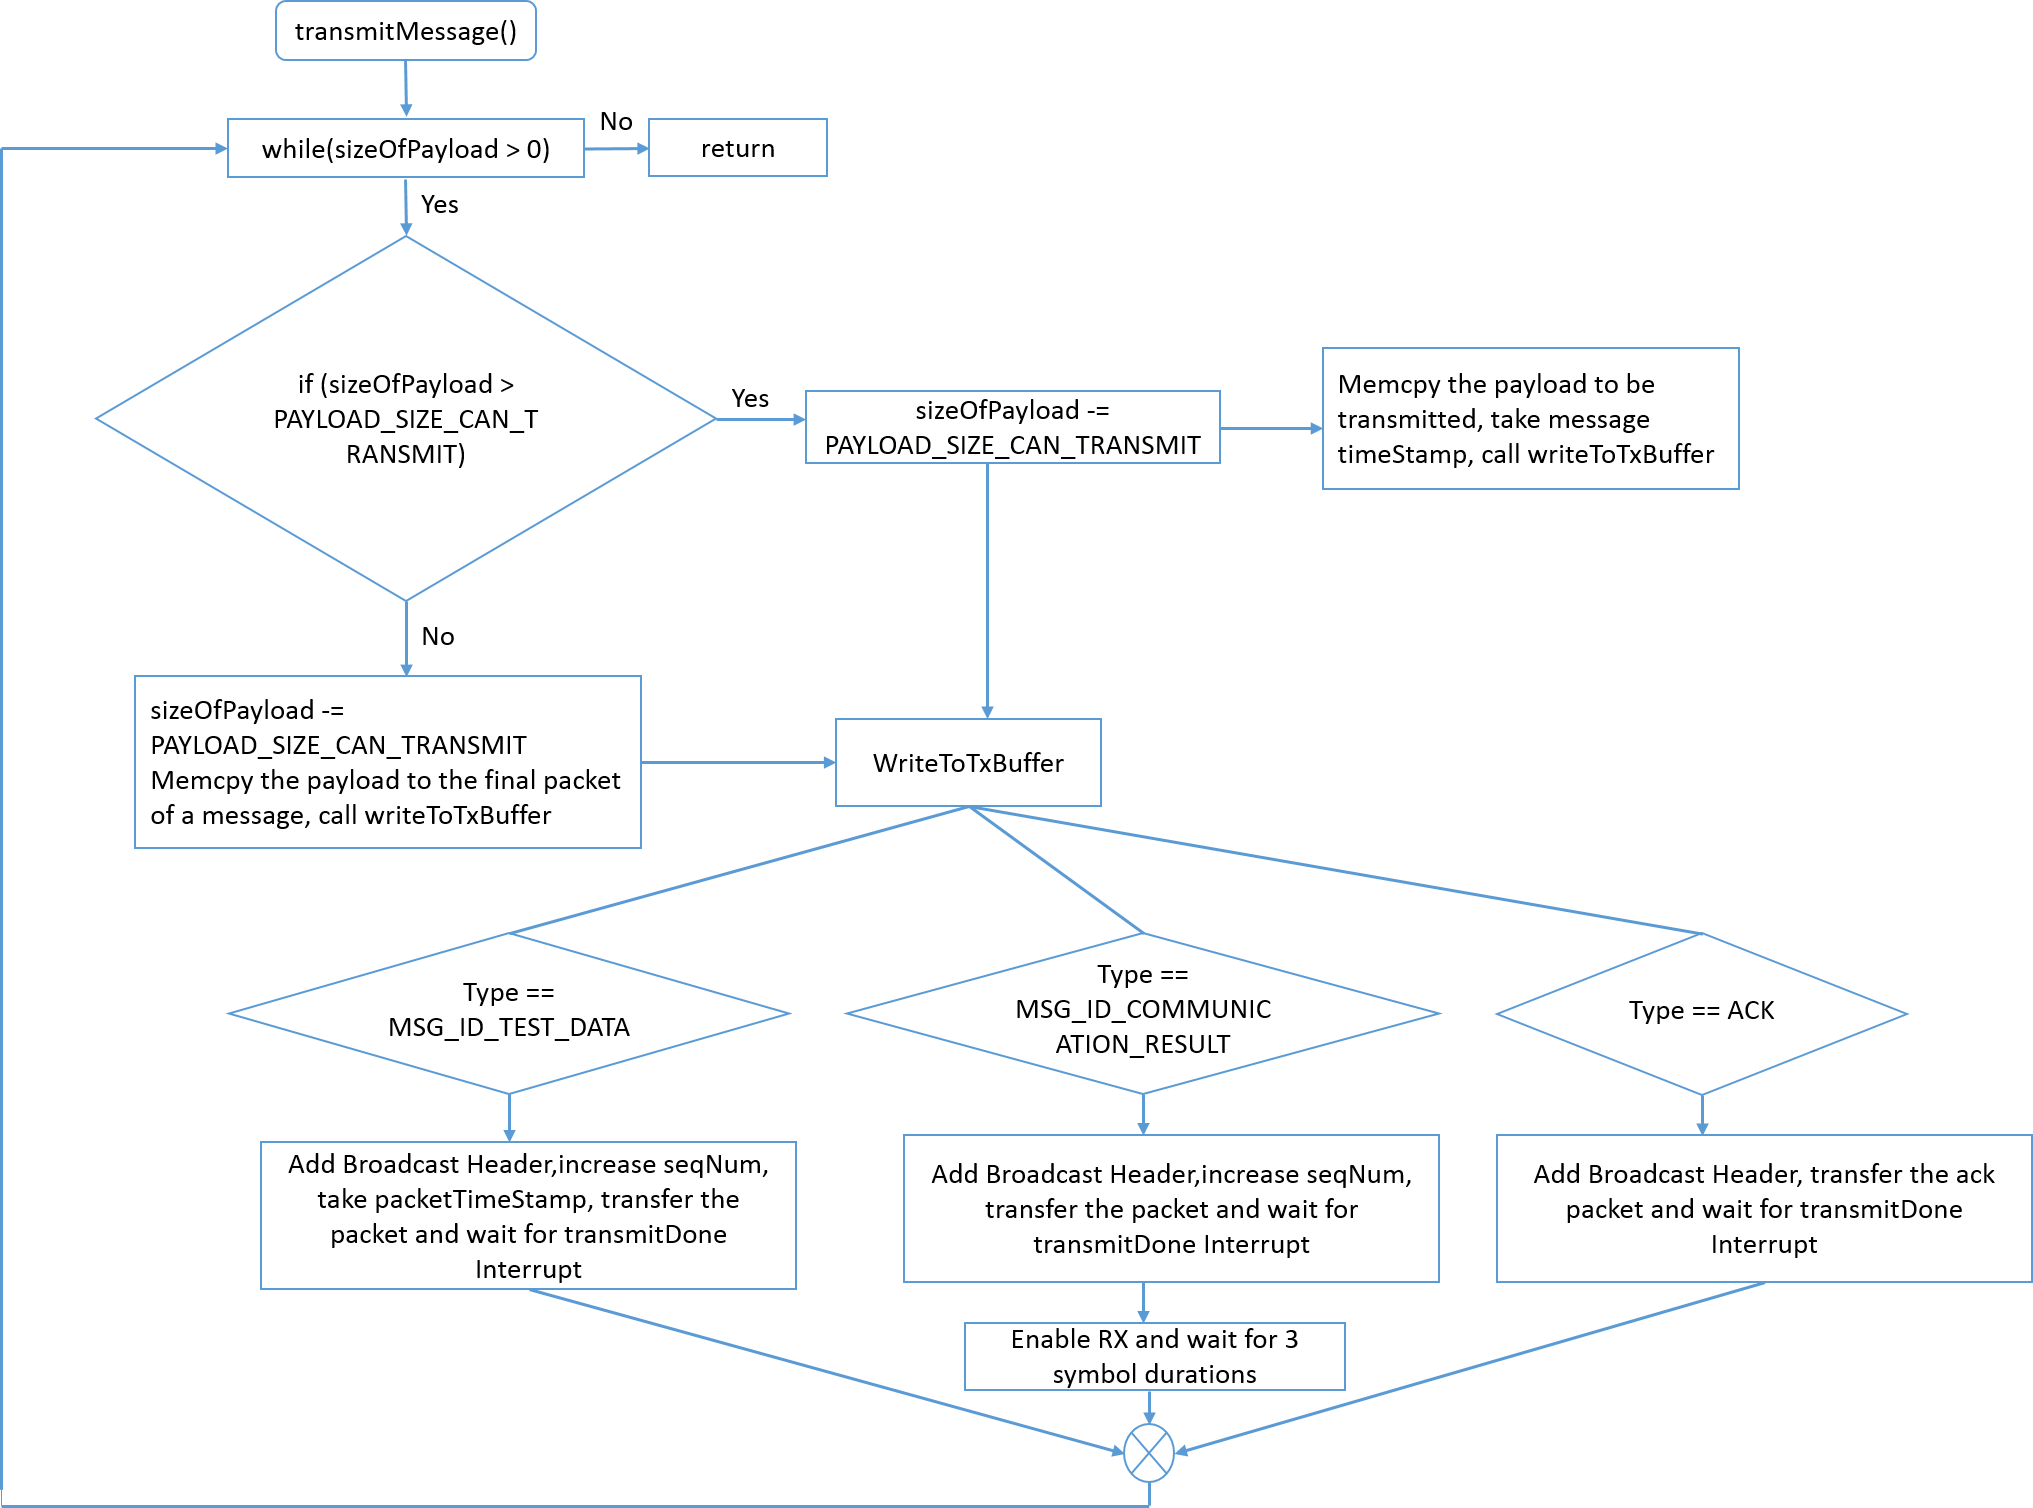
\includegraphics[width=1\textwidth]{figures/transmitMessage}
	\centering
	\caption{Process of transmission of a message}
	\label{fig:transmitMessage}    
\end{figure}
\begin{figure}[h!]
	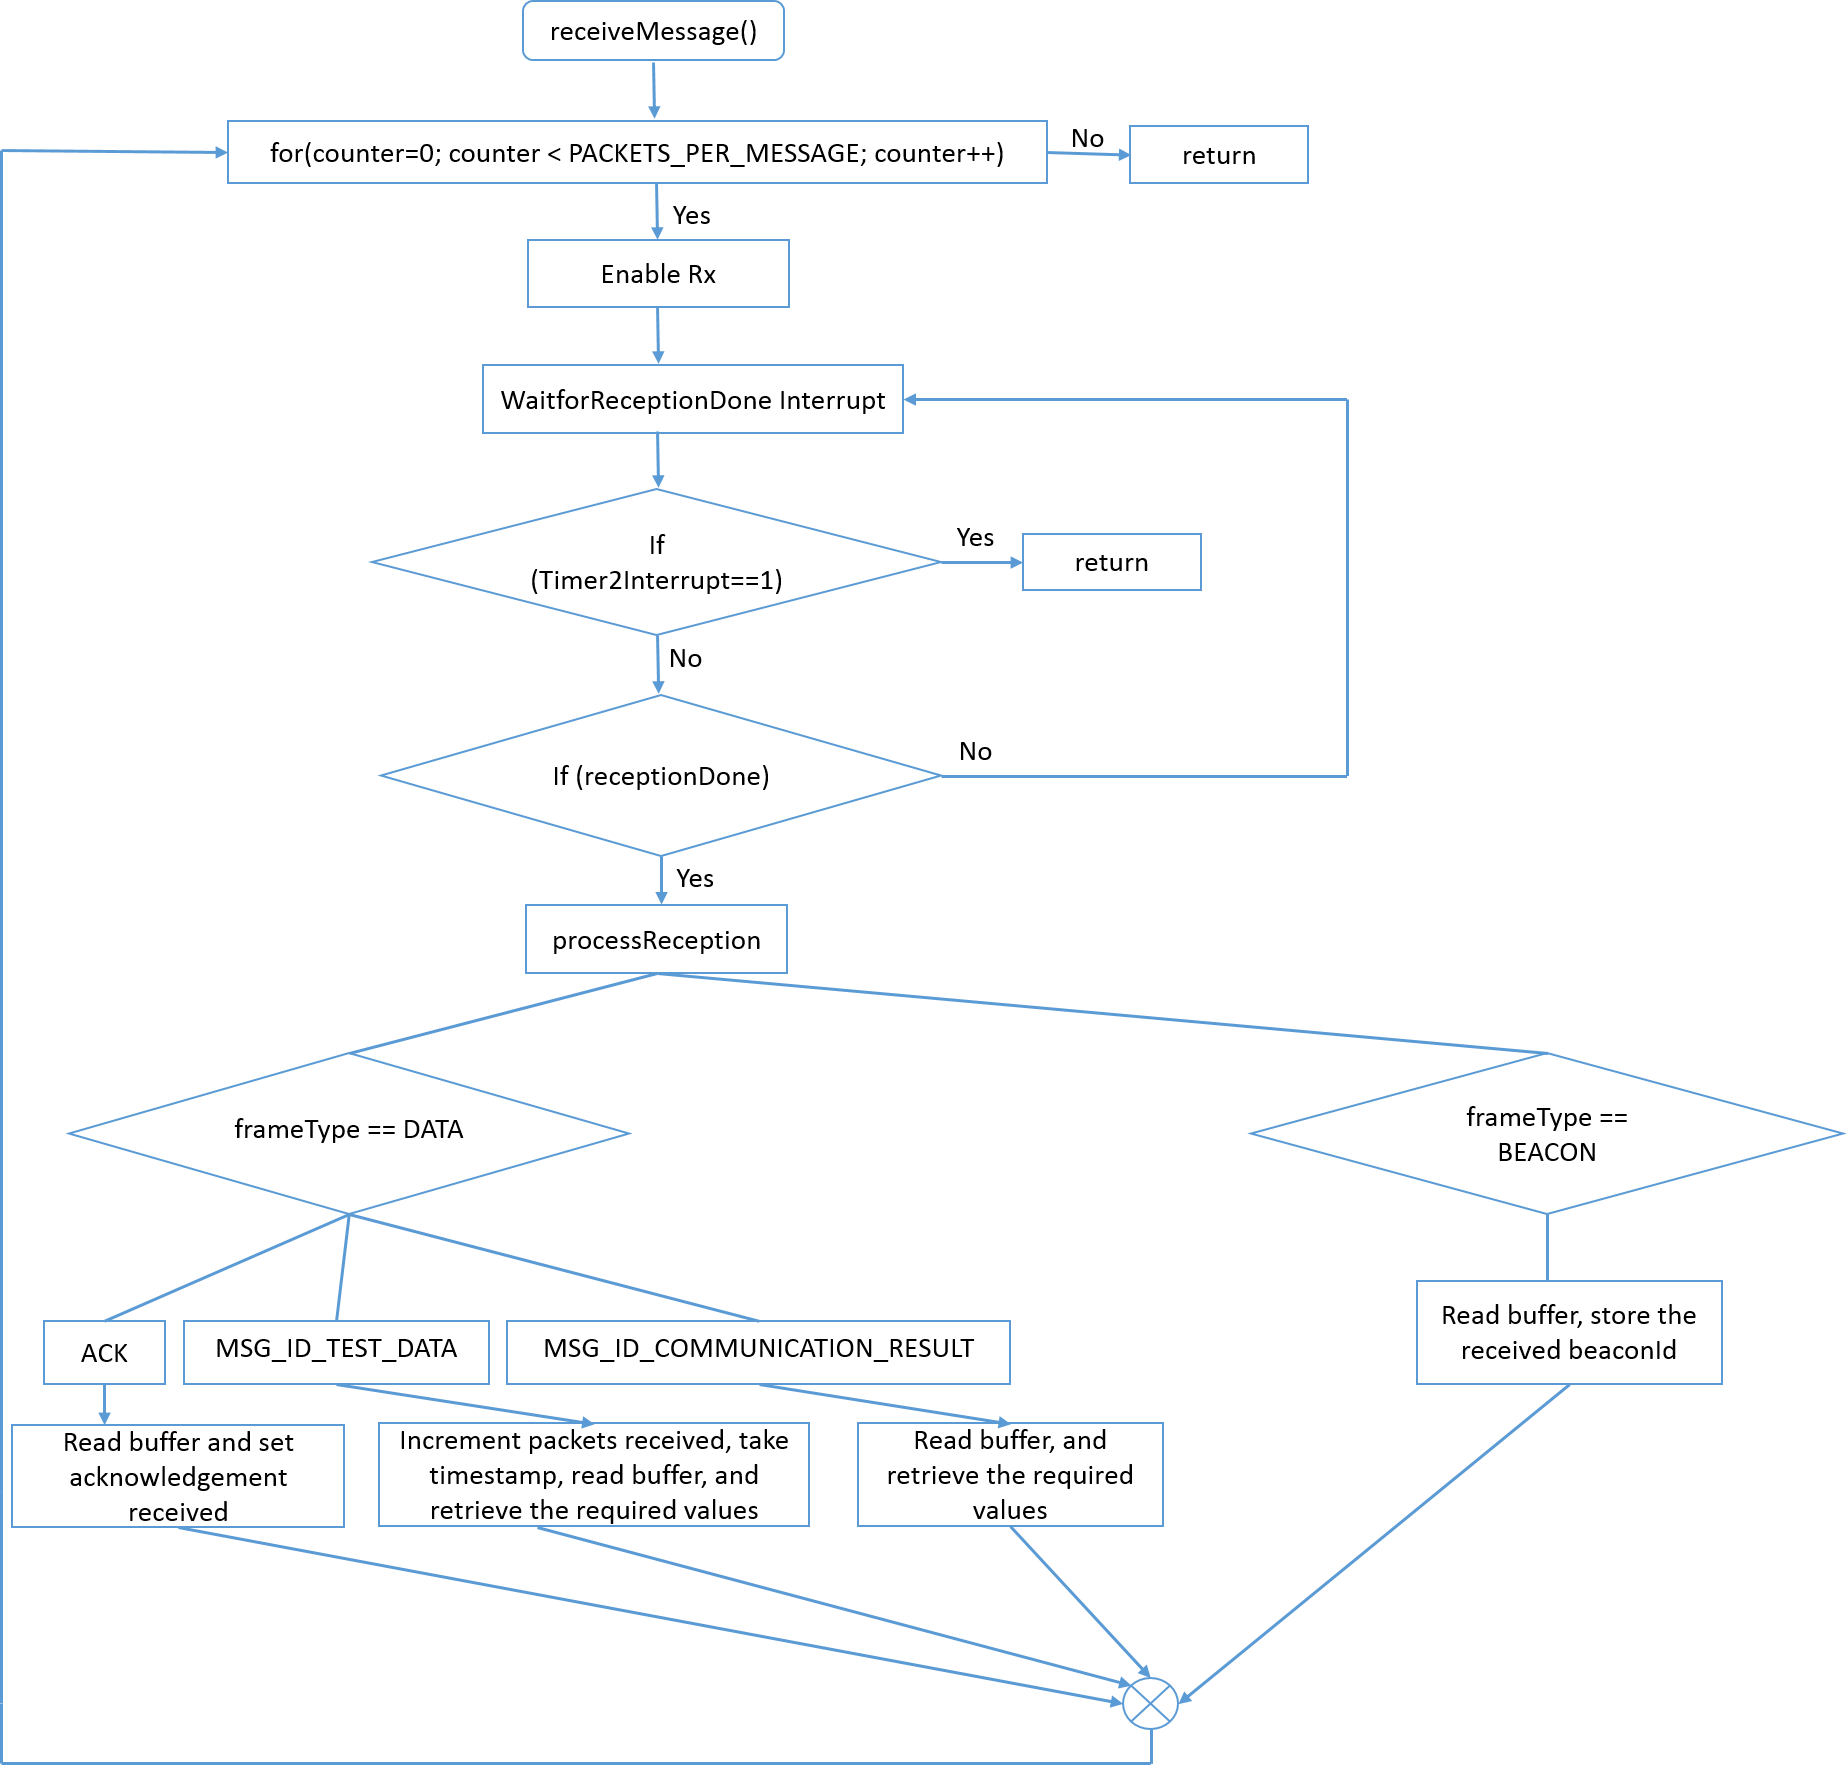
\includegraphics[width=1\textwidth]{figures/receiveMessage}
	\centering
	\caption{Process of reception of a message}
	\label{fig:receiveMessage}    
\end{figure}

\subsubsection{Transmission}
Now, let's consider in detail how the transmission works in the leading truck and the following truck which is indicated in the Figure \ref{fig:transmitMessage}. Inside a while loop, we check if the size of the payload is greater than 0. If so, we split the message into several 127-byte packets according to the IEEE 802.15.4 standard, copy the parts of a message appropriately to individual packets, take message timestamp and call \emph{writeToTxBuffer}. In \emph{writeToTxBuffer}, the transmission of MSG ID TEST DATA, MSG ID COMMUNICATION RESULT, and acknowledgment are handled in different ways. In the case of MSG ID TEST DATA we add the broadcast header, increase the sequence number, take the packet timestamp, transfer the packet and wait for the trasmitDone interrupt. In the case of MSG ID COMMUNICATION RESULT we add the broadcast header, increase the sequence number, transfer the packet and wait for the transmitDone Interrupt. Consequently, we enable RX and wait for three symbol durations for the reception of the acknowledgment. In the case of ACK, we add the broadcast header, transfer the acknowledgment packet and wait for the transmitDone interrupt. Once the size of the payload becomes 0, we exit from the while loop. In between two transmissions, we wait for 2 ms for successful reception of a packet at the receiver.


\subsubsection{Reception}
Figure \ref{fig:receiveMessage} shows how the reception is implemented. When the \emph{receiveMessage()} function is called, we enable the receiver for the first packet of a message and wait for the receptionDone interrupt. While waiting for the receptionDone interrupt, if the Timer2 interrupt occurs which indicates the reception timeout for that particular slot, we return and wait for the Timer1 interrupt, following which we transmit the next message according to the schedule. On the successful reception of the first packet of the message, we process the reception according to the type of the packet received. Since we can only differentiate between the BEACON and DATA message type, we identify the acknowledgment packet, test data and result communication packets based on the global volatile variables: acknow, final=false and final=true respectively. On reception of an acknowledgment packet, we read the buffer and set acknowledgment received to one. On the reception of a test data packet, we increment the number of packets received, take the time stamp, read the buffer and retrieve the required values. On the reception of communication result packet, we read the buffer and retrieve the required values. In the case of reception of a beacon packet, we read the buffer and store the received \emph{beaconId}. Once the reception of the first packet is processed, we enable reception for the second packet of a message, and the process repeats for all packets of a message and returns once all packets of a message are received or if the Timer2 interrupt occurs.

\subsubsection{Latency Calculation}    
We make use of Timer3 for the latency calculation. Figure \ref{fig:latencyCalculationLeadingTruck} and Figure \ref{fig:latencyCalculationFollowingTruck} show the latency calculation for the leading truck and following truck respectively. In order to obtain the message latency, we take the timestamp of the first packet of a message in the application layer before \emph{writeToTxBuffer} function is called and we take the timestamp of the last packet of a message in the application layer after obtaining its payloads, and take the difference between them.

For packet latency, we take the timestamp in the link layer for every packet, in the function \emph{writeToTxBuffer} before copying the payload to the broadcast payload, following which it is written to the transfer buffer and transmission started.  We take the timestamp in the link layer once the same packet has reached the other node, in the function \emph{processReception} that is called after a reception interrupt is handled. 

In Figure \ref{fig:latencyCalculationLeadingTruck}, the x-axis denotes the time, the top part of the figure indicates the leading truck and the bottom part of the figure indicates the following truck. The figure depicts the scenario of two packets per message being sent from the leading truck to the following truck. The message latency is the difference of timestamp $t6$ in the following truck and timestamp $t1$ in the leading truck. The packet latency is the difference of timestamp $t4$ in the following truck and timestamp $t2$ in the leading truck or difference of timestamp $t5$ in the following truck and timestamp $t3$ in the leading truck.

Similarly, the calculation of message latency and packet latency for the following truck is shown in the Figure \ref{fig:latencyCalculationFollowingTruck} wherein a message is transmitted from the following truck to the leading truck.
\begin{figure}[h!]
    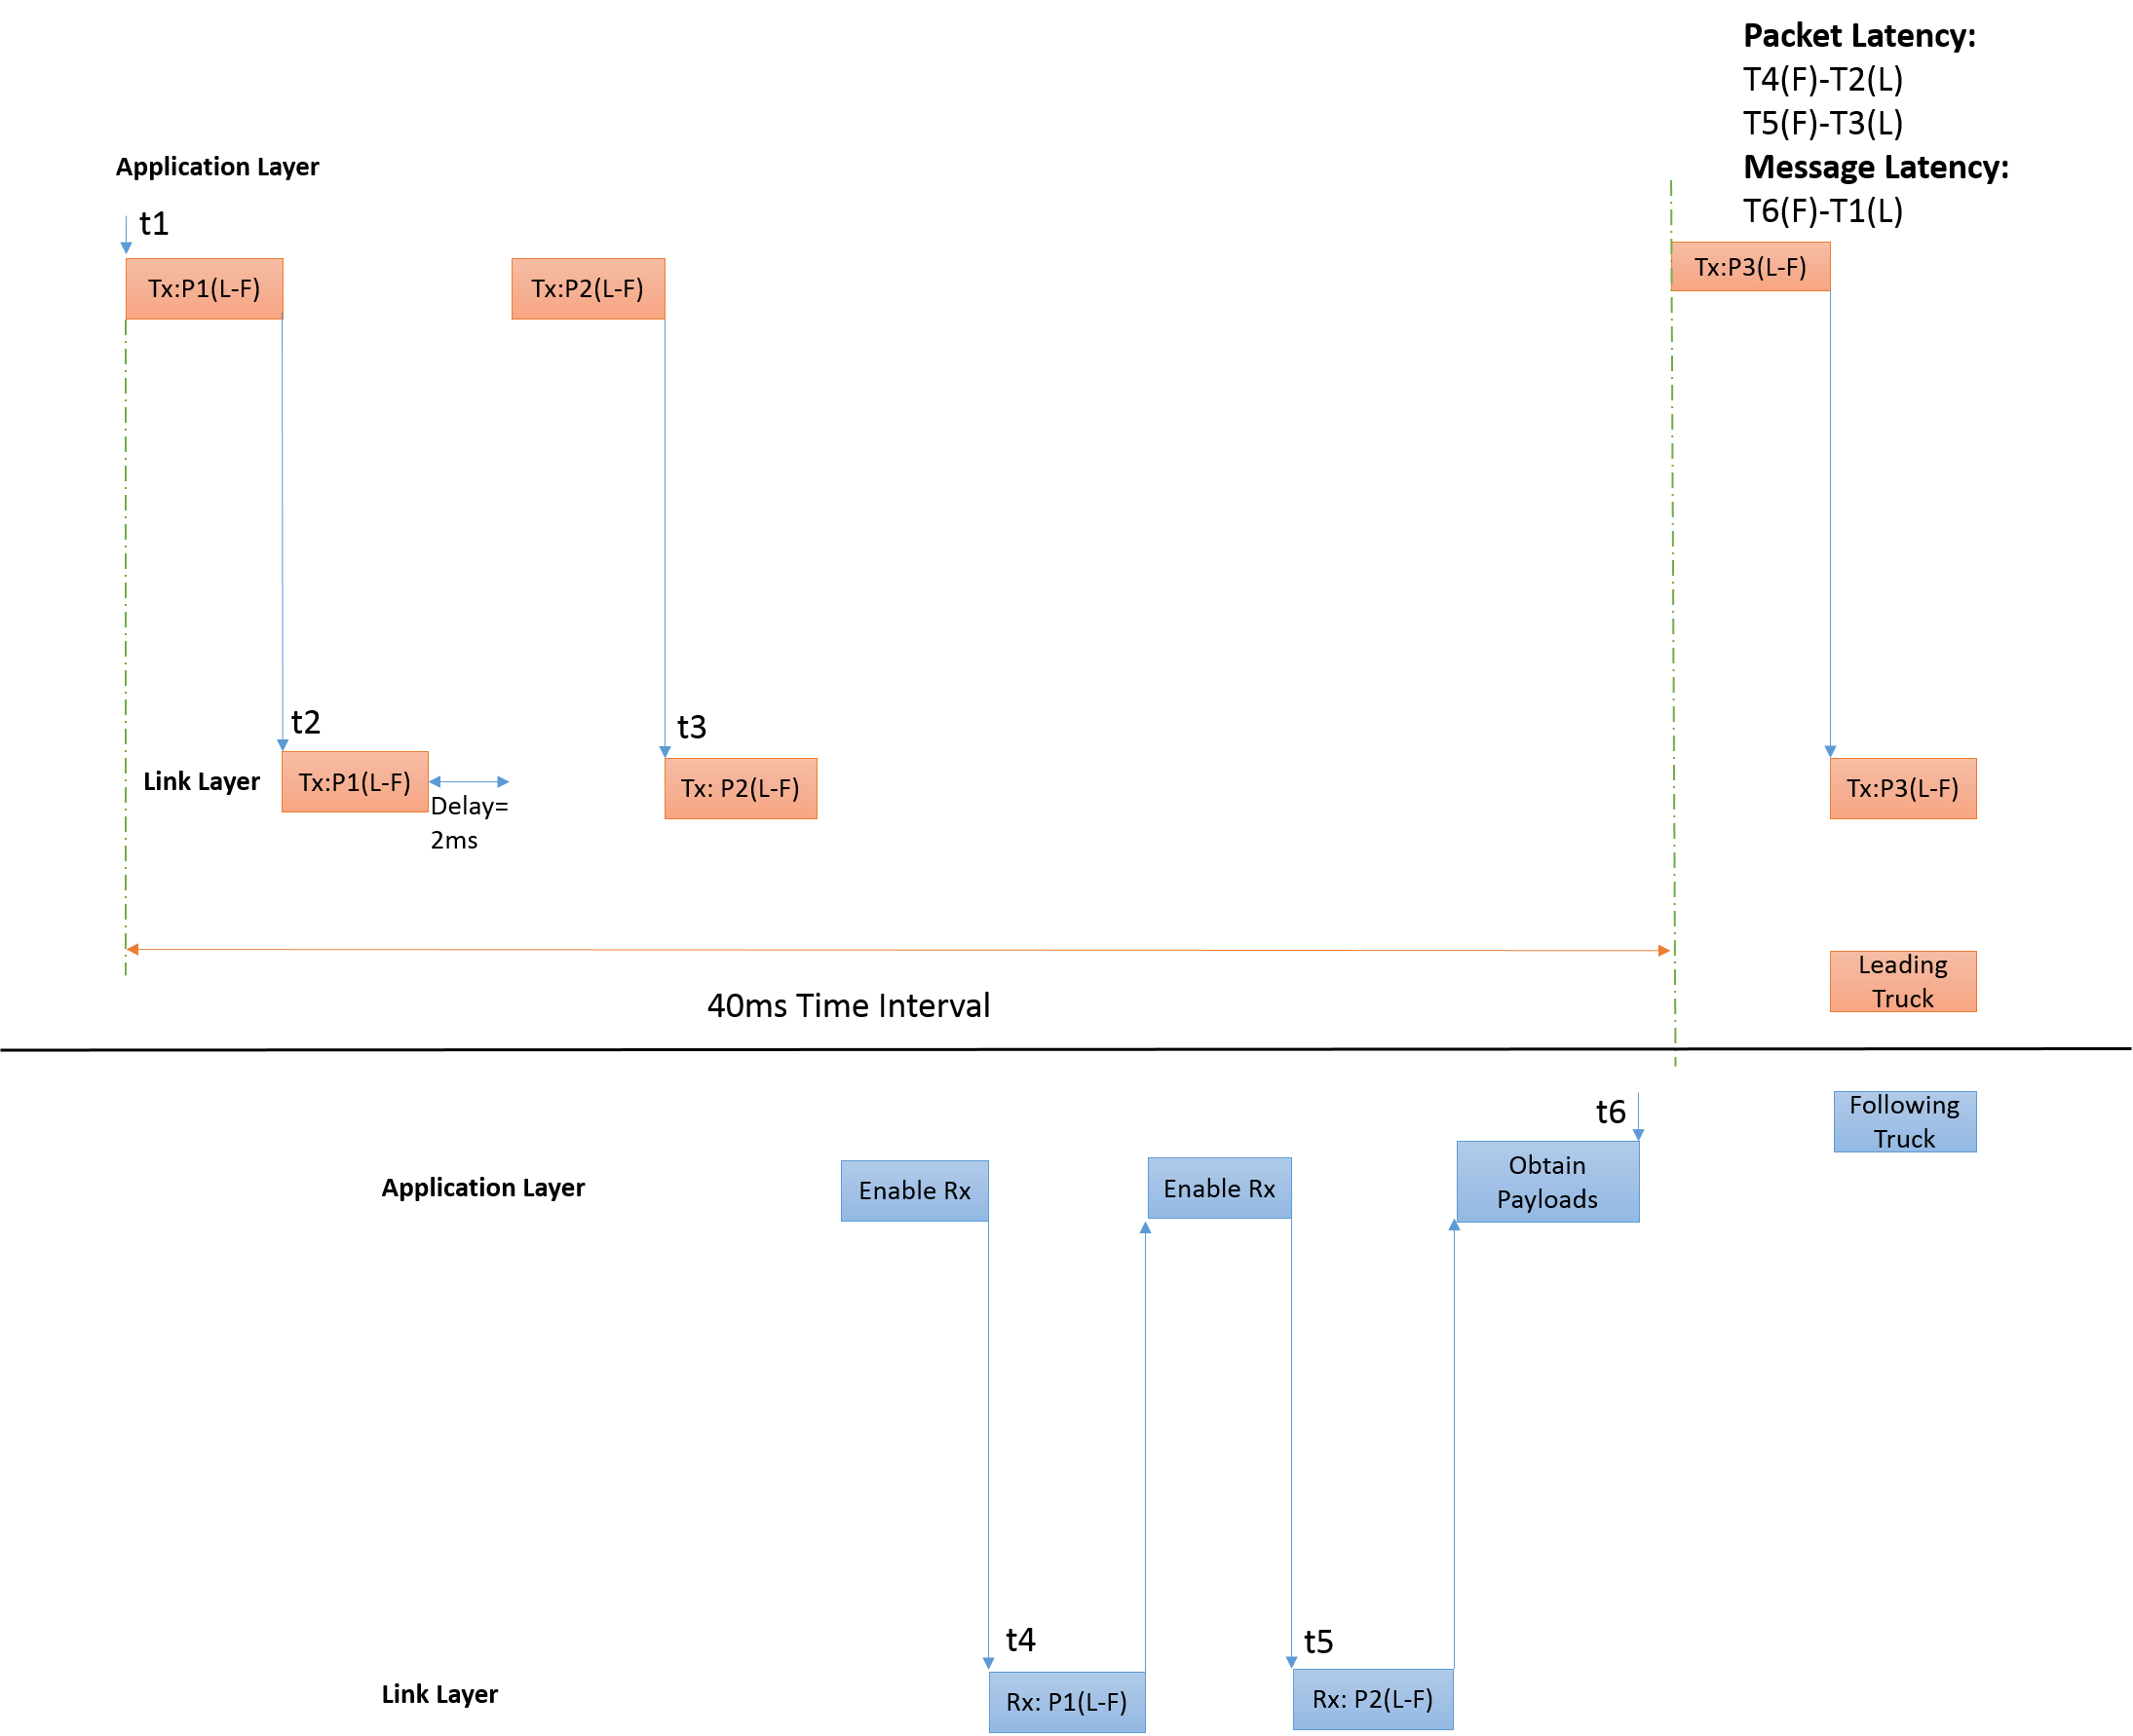
\includegraphics[width=1\textwidth]{figures/LatencyCalculationLeadingTruck}
    \centering
    \caption{Latency Calculation - Leading Truck}
    \label{fig:latencyCalculationLeadingTruck}    
\end{figure}

\begin{figure}[h!]
	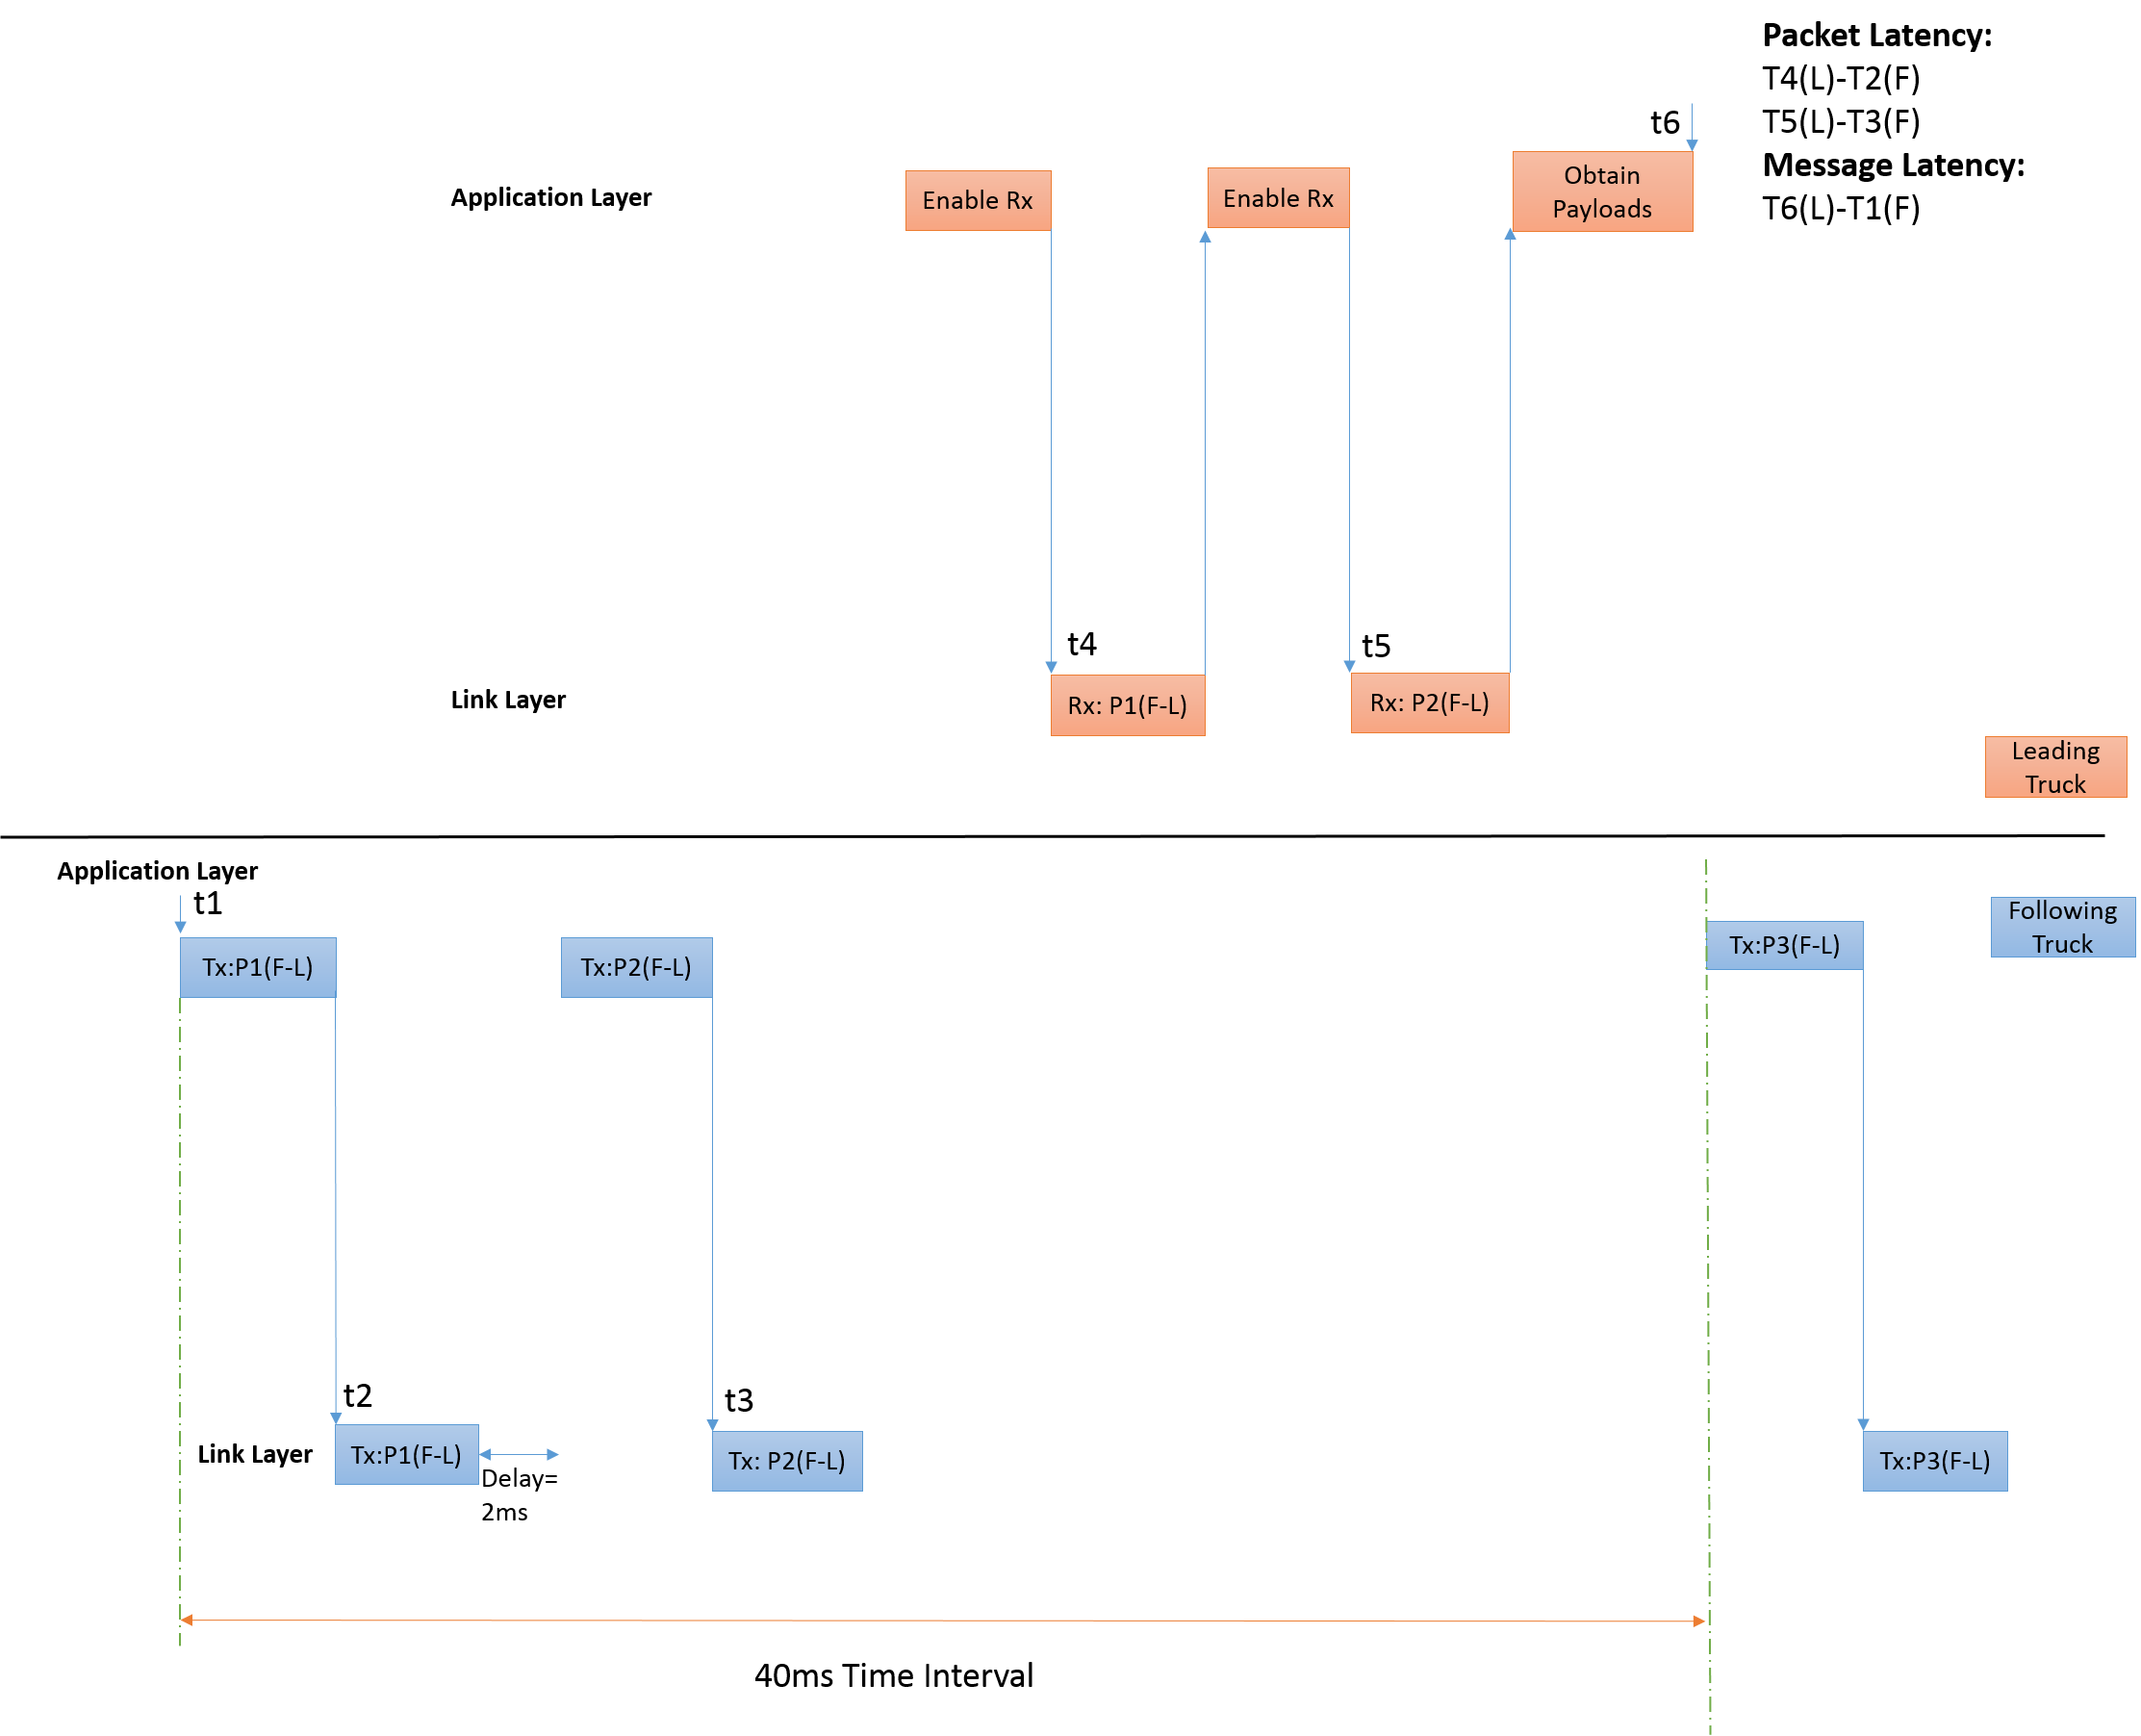
\includegraphics[width=1\textwidth]{figures/LatencyCalculationFollowingTruck}
	\centering
	\caption{Latency Calculation - Following Truck}
	\label{fig:latencyCalculationFollowingTruck}    
\end{figure}

\begin{figure}[h!]
	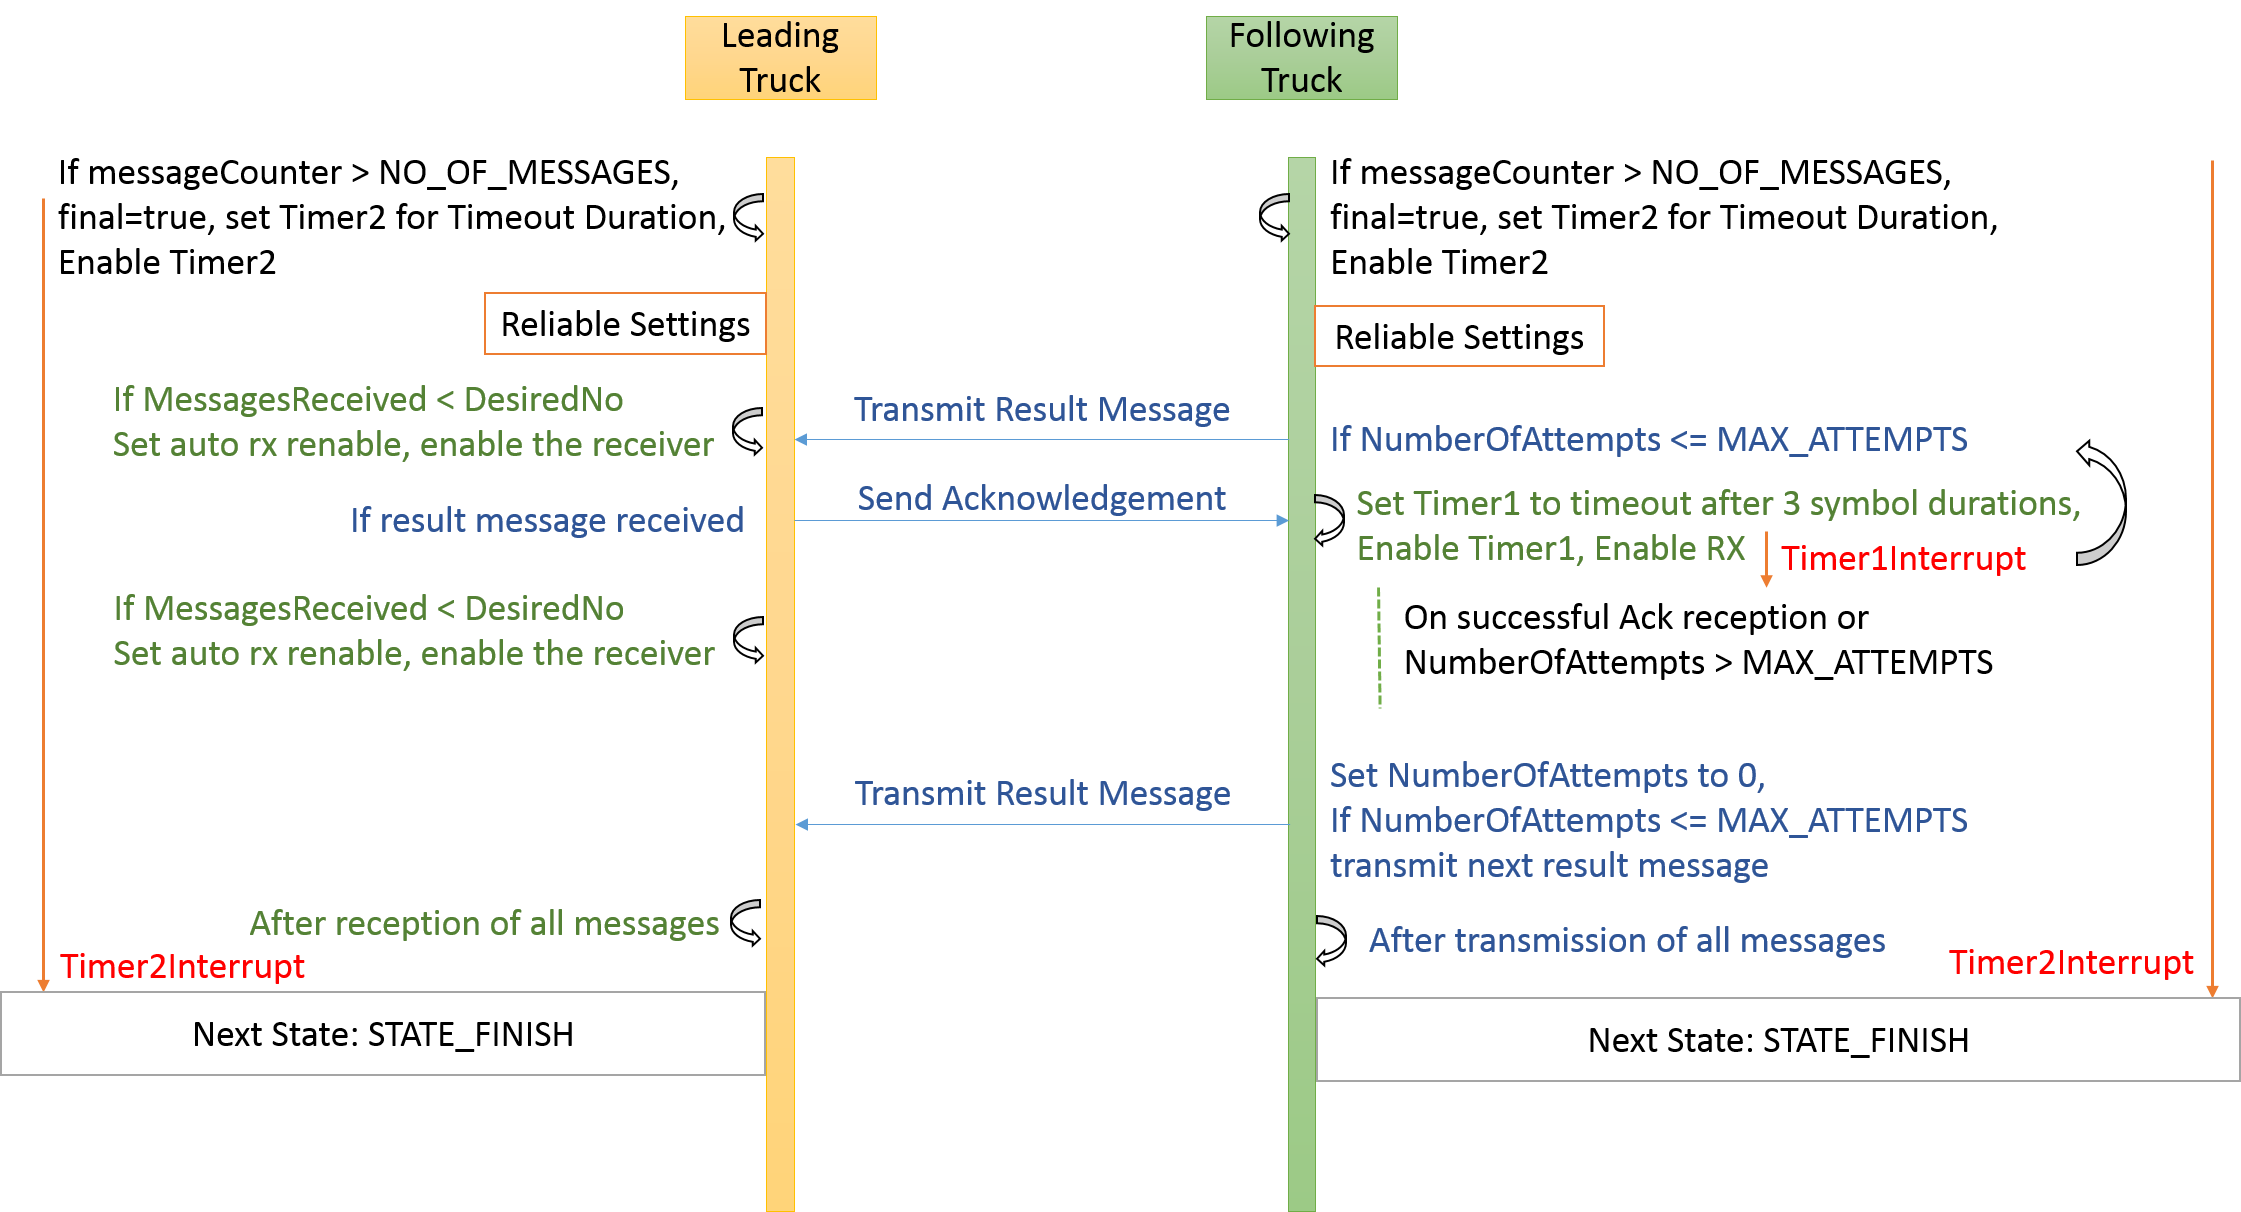
\includegraphics[width=1\textwidth]{figures/StateResultDetermination}
	\centering
	\caption{State Result Determination}
	\label{fig:StateResultDetermination}    
\end{figure}

\subsection{State Result Communication}
The working of State Result Communication is indicated in the Figure \ref{fig:StateResultDetermination}. If messageCounter \textgreater \emph{NO\_OF\_MESSAGES}, we set final=true and enter State Result Communication in both nodes. It is to be noted that the leading truck enters this state earlier than the following truck because of the 20 ms offset in the following truck. We set Timer2 for the timeout duration for the entire phase and enable timer2. We make use of the reliable settings in this phase, wherein we use the lowest data rate of 110 kbps and make use of acknowledgment for each log sent in this phase. 

In the case of the following truck, for a particular log, we define \emph{MAX\_ATTEMPTS} as the number of times to repeat sending that particular log until an acknowledgment is received. If the number of attempts is less than or equal to the \emph{MAX\_ATTEMPTS}, we transmit that particular log. Following which, we set Timer1 to timeout after three symbol durations, enable Timer1 and enable receiver for the reception of acknowledgment. On the occurrence of Timer1 interrupt, we increment the number of attempts, go back and transmit that particular log again if the number of attempts is less than or equal to the \emph{MAX\_ATTEMPTS}. On the reception of acknowledgment, we set the number of attempts to 0 and transmit the next result log if the number of attempts is less than or equal to \emph{MAX\_ATTEMPTS}. This process continues for all the result logs, and it enters the next phase STATE FINISH after transmission of all logs or if Timer2 interrupt occurs.

In the case of the leading truck, if the number of logs received is less than \emph{DesiredNo} we set \emph{autorxreenable} and enable the receiver. If the result log is received, we process that particular log and send an acknowledgment back. Following which we set \emph{autorxreenable} and enable the receiver if the number of messages received is less than \emph{DesiredNo}. This process continues for the reception of all the logs and it enters the next phase STATE FINISH after the reception of all logs or if Timer2 interrupt occurs. The test log structure definition is shown in Listing \ref{lst:testLogStructureDefinition}. Using the stored values of this structure for each log, a comma separated string is created as shown in Listing \ref{lst:loggingFormat} and printed on the laptop/computer using serial communication, which is further processed in MATLAB.

\begin{lstlisting}[caption={Logging Format},
label={lst:loggingFormat}, language=C]
Log,tseqno1,0,tseqno2,1,tseqno3,2,tseqno4,3,rseqno1,0,rseqno2,1,rseqno3,2,rseqno4,3,messageLatency,8.950,packetLatency1,0.843,packetLatency2,0.843,packetLatency3,0.843,packetLatency4,0.829,distance,0.00,C1,955,C2,1015,C3,1028,C4,925,N1,236,N2,236,N3,235,N4,229,F11,2716,F12,2385,F13,2883,F14,2420,F21,3033,F22,3369,F23,3040,F24,3099,F31,2971,F32,2439,F33,2869,F34,2290
\end{lstlisting}

\vspace{2cm}
\begin{lstlisting}[caption={Test Log structure definition}, label={lst:testLogStructureDefinition}, language=C]
typedef struct {
uint16_t tseqNo[PACKETS_PER_MESSAGE];
uint16_t rseqNo[PACKETS_PER_MESSAGE];
uint32_t messageLatency;
uint32_t packetLatency[PACKETS_PER_MESSAGE];
double distance;
uint16_t stdNoise[PACKETS_PER_MESSAGE];
uint16_t C[PACKETS_PER_MESSAGE];
uint16_t N[PACKETS_PER_MESSAGE];
uint16_t F1[PACKETS_PER_MESSAGE];
uint16_t F2[PACKETS_PER_MESSAGE];
uint16_t F3[PACKETS_PER_MESSAGE];
}logging;
\end{lstlisting}





\subsection{State Finish}
In the phase STATE FINISH, we reset for the next configuration and stop the link. Wherein we disable all interrupts which were set in STATE START, disable all the three timers, reset them and reset the transceiver. If the number of times to repeat is less than (NO OF TIMES TO RUN * NUM OF DW1000 CONFIGS) we load the next configuration ((configuration + 1) \% NUM OF DW1000 CONFIGS) and return to STATE START, else we stop the execution.

\subsection{Ranging Method}
For the implementation of ranging, we make use of Double-Sided Two-Way Ranging (DS-TWR), which is an extension of the basic single-sided two-way ranging in which two round trip time measurements are used and combined to give a time-of-flight result which has a reduced error even for quite long response delays. The operation of DS-TWR used in our implementation is shown in Figure \ref{fig:rangingMethod}. The leading truck sends a POLL packet to the following truck, for which the following truck sends a response packet to the leading truck. Consequently, the leading truck sends a final packet to the following truck. Lastly, the following truck sends the result packet to the leading truck with all the required time stamps from the following truck (POLL RX time stamp, RESPONSE TX time stamp and FINAL RX time stamp). The leading truck makes use of the time stamps sent in the result packet and its own time stamps (POLL TX time stamp, RESPONSE RX time stamp and FINAL TX time stamp) to calculate the time-of-flight estimate according to  Equation \ref{eq:tofestimate}. Using this time-of-flight estimate, distance is calculated according to  Equation \ref{eq:distanceEstimate}.

\begin{equation}
\label{eq:tofestimate}
T_{prop}=\dfrac{T_{round1}*T_{round2}-T_{reply1}*T_{reply2}}{T_{round1}+T_{round2}+T_{reply1}+T_{reply2}}
\end{equation}

\begin{equation}
\label{eq:distanceEstimate}
Distance = T_{prop} * SPEED\_OF\_LIGHT
\end{equation}

\begin{figure}[h!]
    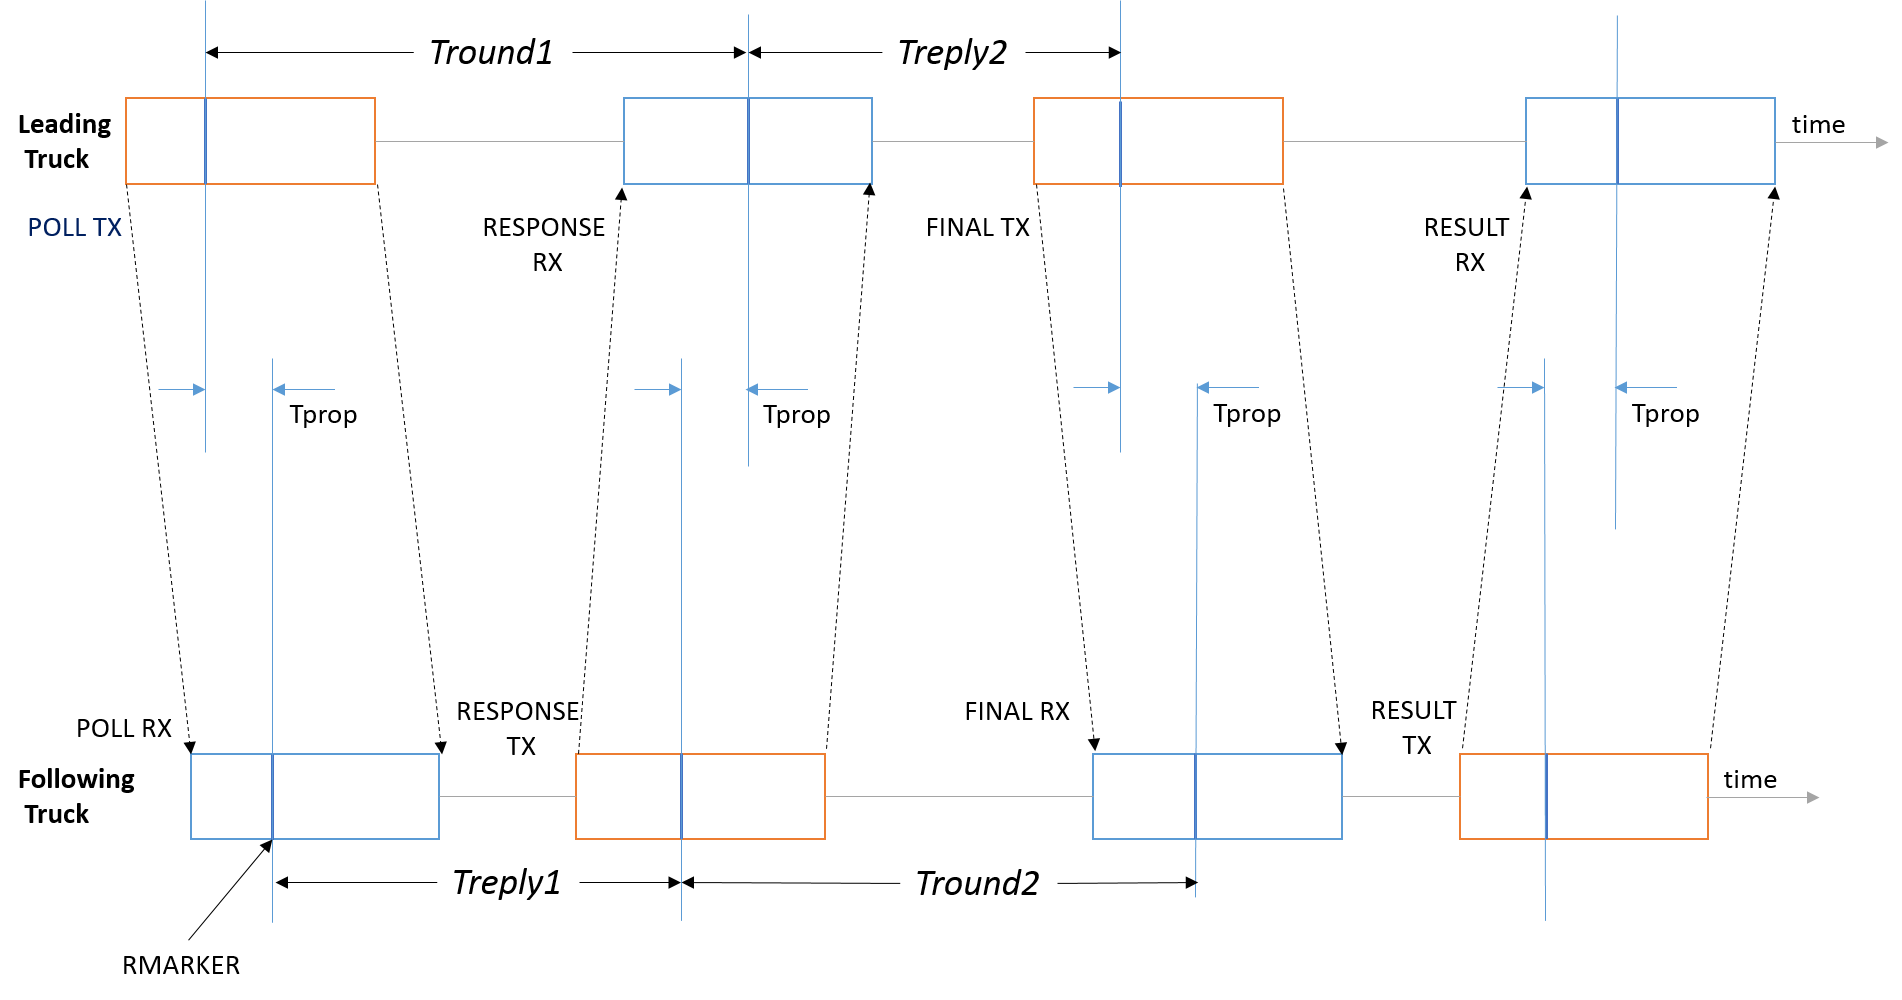
\includegraphics[width=1\textwidth]{figures/RangingMethod}
    \centering
    \caption{Ranging Method}
    \label{fig:rangingMethod}    
\end{figure}

\subsection{Ranging Implementation}
Figure \ref{fig:implementationOfRanging} shows how we integrate ranging along with communication. We refer to the last packet of a message to send/receive ranging related information. Initially, we reset the parameters for range calculation in both the leading truck and the following truck. 

In the case of the following truck, on the reception of ranging POLL information, it resets the parameters and gets the POLL RX time stamp. It sends the ranging RESPONSE information when \emph{rangeType}\%2==0. On the reception of the ranging FINAL information, it gets the RESPONSE TX time stamp and the FINAL RX time stamp. It sends the ranging RESULT information along with the POLL RX time stamp, the RESPONSE TX time stamp and the FINAL RX time stamp when \emph{rangeType}\%2==1.

In the case of the leading truck, it sends the Ranging POLL information when \emph{rangeType}\%2==0. On reception of the ranging RESPONSE information from the following truck, it resets the parameters and gets the POLL TX time stamp and the RESPONSE RX time stamp. It sends the ranging FINAL information when \emph{rangeType}\%2==1. On reception of the ranging RESULT information from the following truck, it gets the FINAL TX time stamp, retrieves the POLL RX time stamp, the RESPONSE TX time stamp and the FINAL RX time stamp from the ranging RESULT information and calculates the distance between the trucks. The reset of the parameters is done to ensure the distance is calculated appropriately even in the case of packet loss. To calculate the distance, the time-of-flight estimate calculated according to the equation \ref{eq:tofestimate} is multiplied by DWT TIME UNITS since these time stamps are given by the DecaWave device and finally the distance is calculated according to the equation \ref{eq:distanceEstimate}.
   
\begin{figure}[h!]
    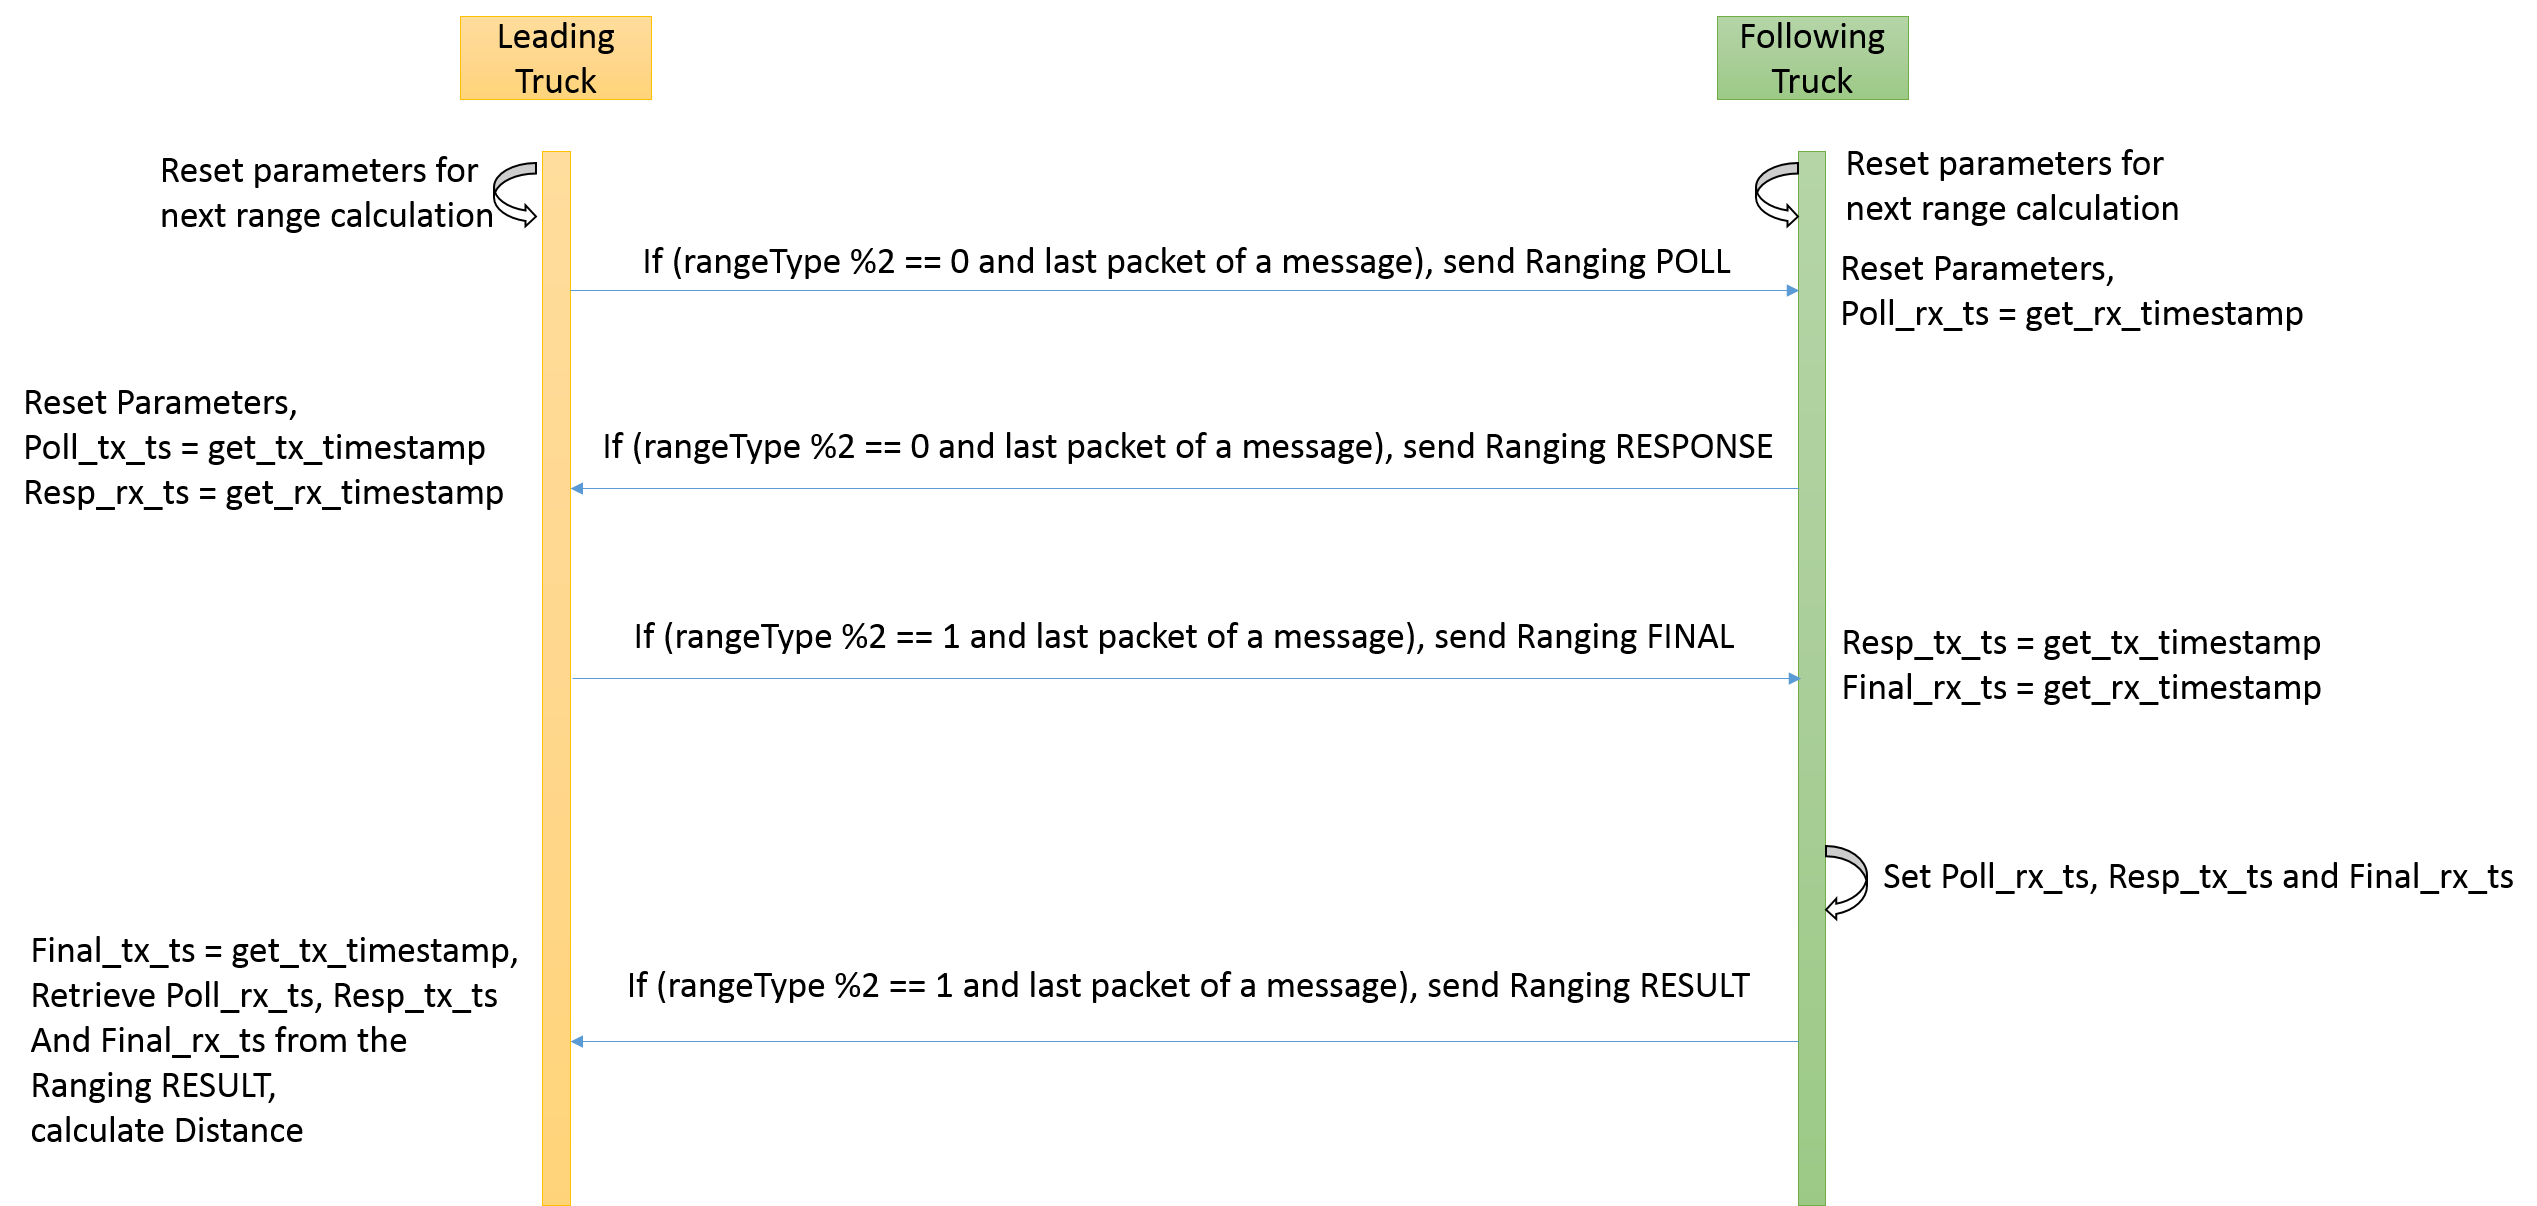
\includegraphics[width=1\textwidth]{figures/RangingCalculation}
    \centering
    \caption{Implementation of Ranging}
    \label{fig:implementationOfRanging}    
\end{figure}

\vspace{2cm}

\subsection{Cross Verification of Design}

To cross verify if the system is designed accurately, additional parameters were logged for the packets as shown in Listing \ref{lst:testLogStructureVerificationOfDesign} in the unit testing phase. An indication of the parameters logged is provided in Figure \ref{fig:LoggedParametersDetermineAppWorking}. 
\begin{lstlisting}[caption={Test Log structure for verification of design}, label={lst:testLogStructureVerificationOfDesign}, language=C]
typedef struct {
uint16_t tseqNo[PACKETS_PER_MESSAGE];
uint16_t rseqNo[PACKETS_PER_MESSAGE];
uint32_t tonTimePacket[4];
uint32_t ronTimePacket[4];
uint32_t tcompletiontimePacket[4];
uint32_t rcompletiontimePacket[4];
uint32_t messageLatency;
uint32_t packetLatency[PACKETS_PER_MESSAGE];
uint8_t timeout[PACKETS_PER_MESSAGE];
uint32_t errorcompletiontimePacket[4];
double distance;
uint16_t stdNoise[PACKETS_PER_MESSAGE];
uint16_t C[PACKETS_PER_MESSAGE];
uint16_t N[PACKETS_PER_MESSAGE];
uint16_t F1[PACKETS_PER_MESSAGE];
uint16_t F2[PACKETS_PER_MESSAGE];
uint16_t F3[PACKETS_PER_MESSAGE];
} logging;
\end{lstlisting}
Here the parameter 'timeout' indicates if a timeout occurred during the reception of a packet and 'errorcompletiontimePacket' indicates the timestamp if any errors like Rx Frame timeout, Rx SFD timeout, Rx Preamble timeout, RX PHR error, Rx Reed-Solomon error (Sync loss),or Rx Bad CRC occur. Using these parameters we checked if the receiver of the following truck is turned on before the transmission from the leading truck for every packet of a message and similarly we checked if the receiver of the leading truck is turned on before the transmission from the following truck for every packet of a message. We also checked if the time between the transmission of packets was 2 ms and the time between the reception completion of one packet and enablement of reception for the next packet is less than 2 ms. We verified if the system worked as designed during timeouts or when errors occurred. We also verified that the nodes are synchronized when they enter the communication phase through an oscilloscope by creating a pulse on the GPIO Pin on entering the communication phase. It was observed that the difference in synchronization was less than 200 $\mu$s, which is ok for our application.

During the cross verification of the design, two major issues were found when the code was run for long durations of time. The first issue was that the schedule of transmission was getting affected in few cases wherein the receiver of the following truck was not getting turned on before the transmission of a packet from the leading truck and vice versa. This error was not reproducible and hence it was tough to identify the source of the problem. To solve this problem, flags were used to identify in what phase the node was when Timer1 interrupt of 40 ms occurred. It was observed that the node was always in the logging state when Timer1 occurred. At that point of time when this error occurred, the sequence of the code was to transmit a message, receive a message, log that particular message and then go to the next transmission. Having identified that the issue was associated with logging, we turned off all logging and printed an error only if a packet reception was missed. We found that the code worked as desired. Digging deep into the issue we found that the issue was associated with the COM port interrupts interfering with the Timer1 and Timer2 Interrupts. To solve this issue, we stored all the logging information in a structure array and handled the printing of the log after the communication phase.

Another issue that was identified is that the code crashed at times. This error too was not reproducible. The approach used to solve this issue was to store values of certain variables in RAM and print the values of these variables on pressing reset after the crash occurred. To do this, we changed the settings in LPCXpresso IDE to trick the microcontroller to believe that there is lesser memory space available while creating the makefile and used that part of memory for storing the values of these variables. It was identified that the issue was caused due to the reception of an unexpected packet which could occur if the reception and timeout interrupt occurred at the same point in time. This exception was handled to solve this problem, and the system was cross-verified for the designed functioning before going into the experimentation.

\begin{figure}[h!]
    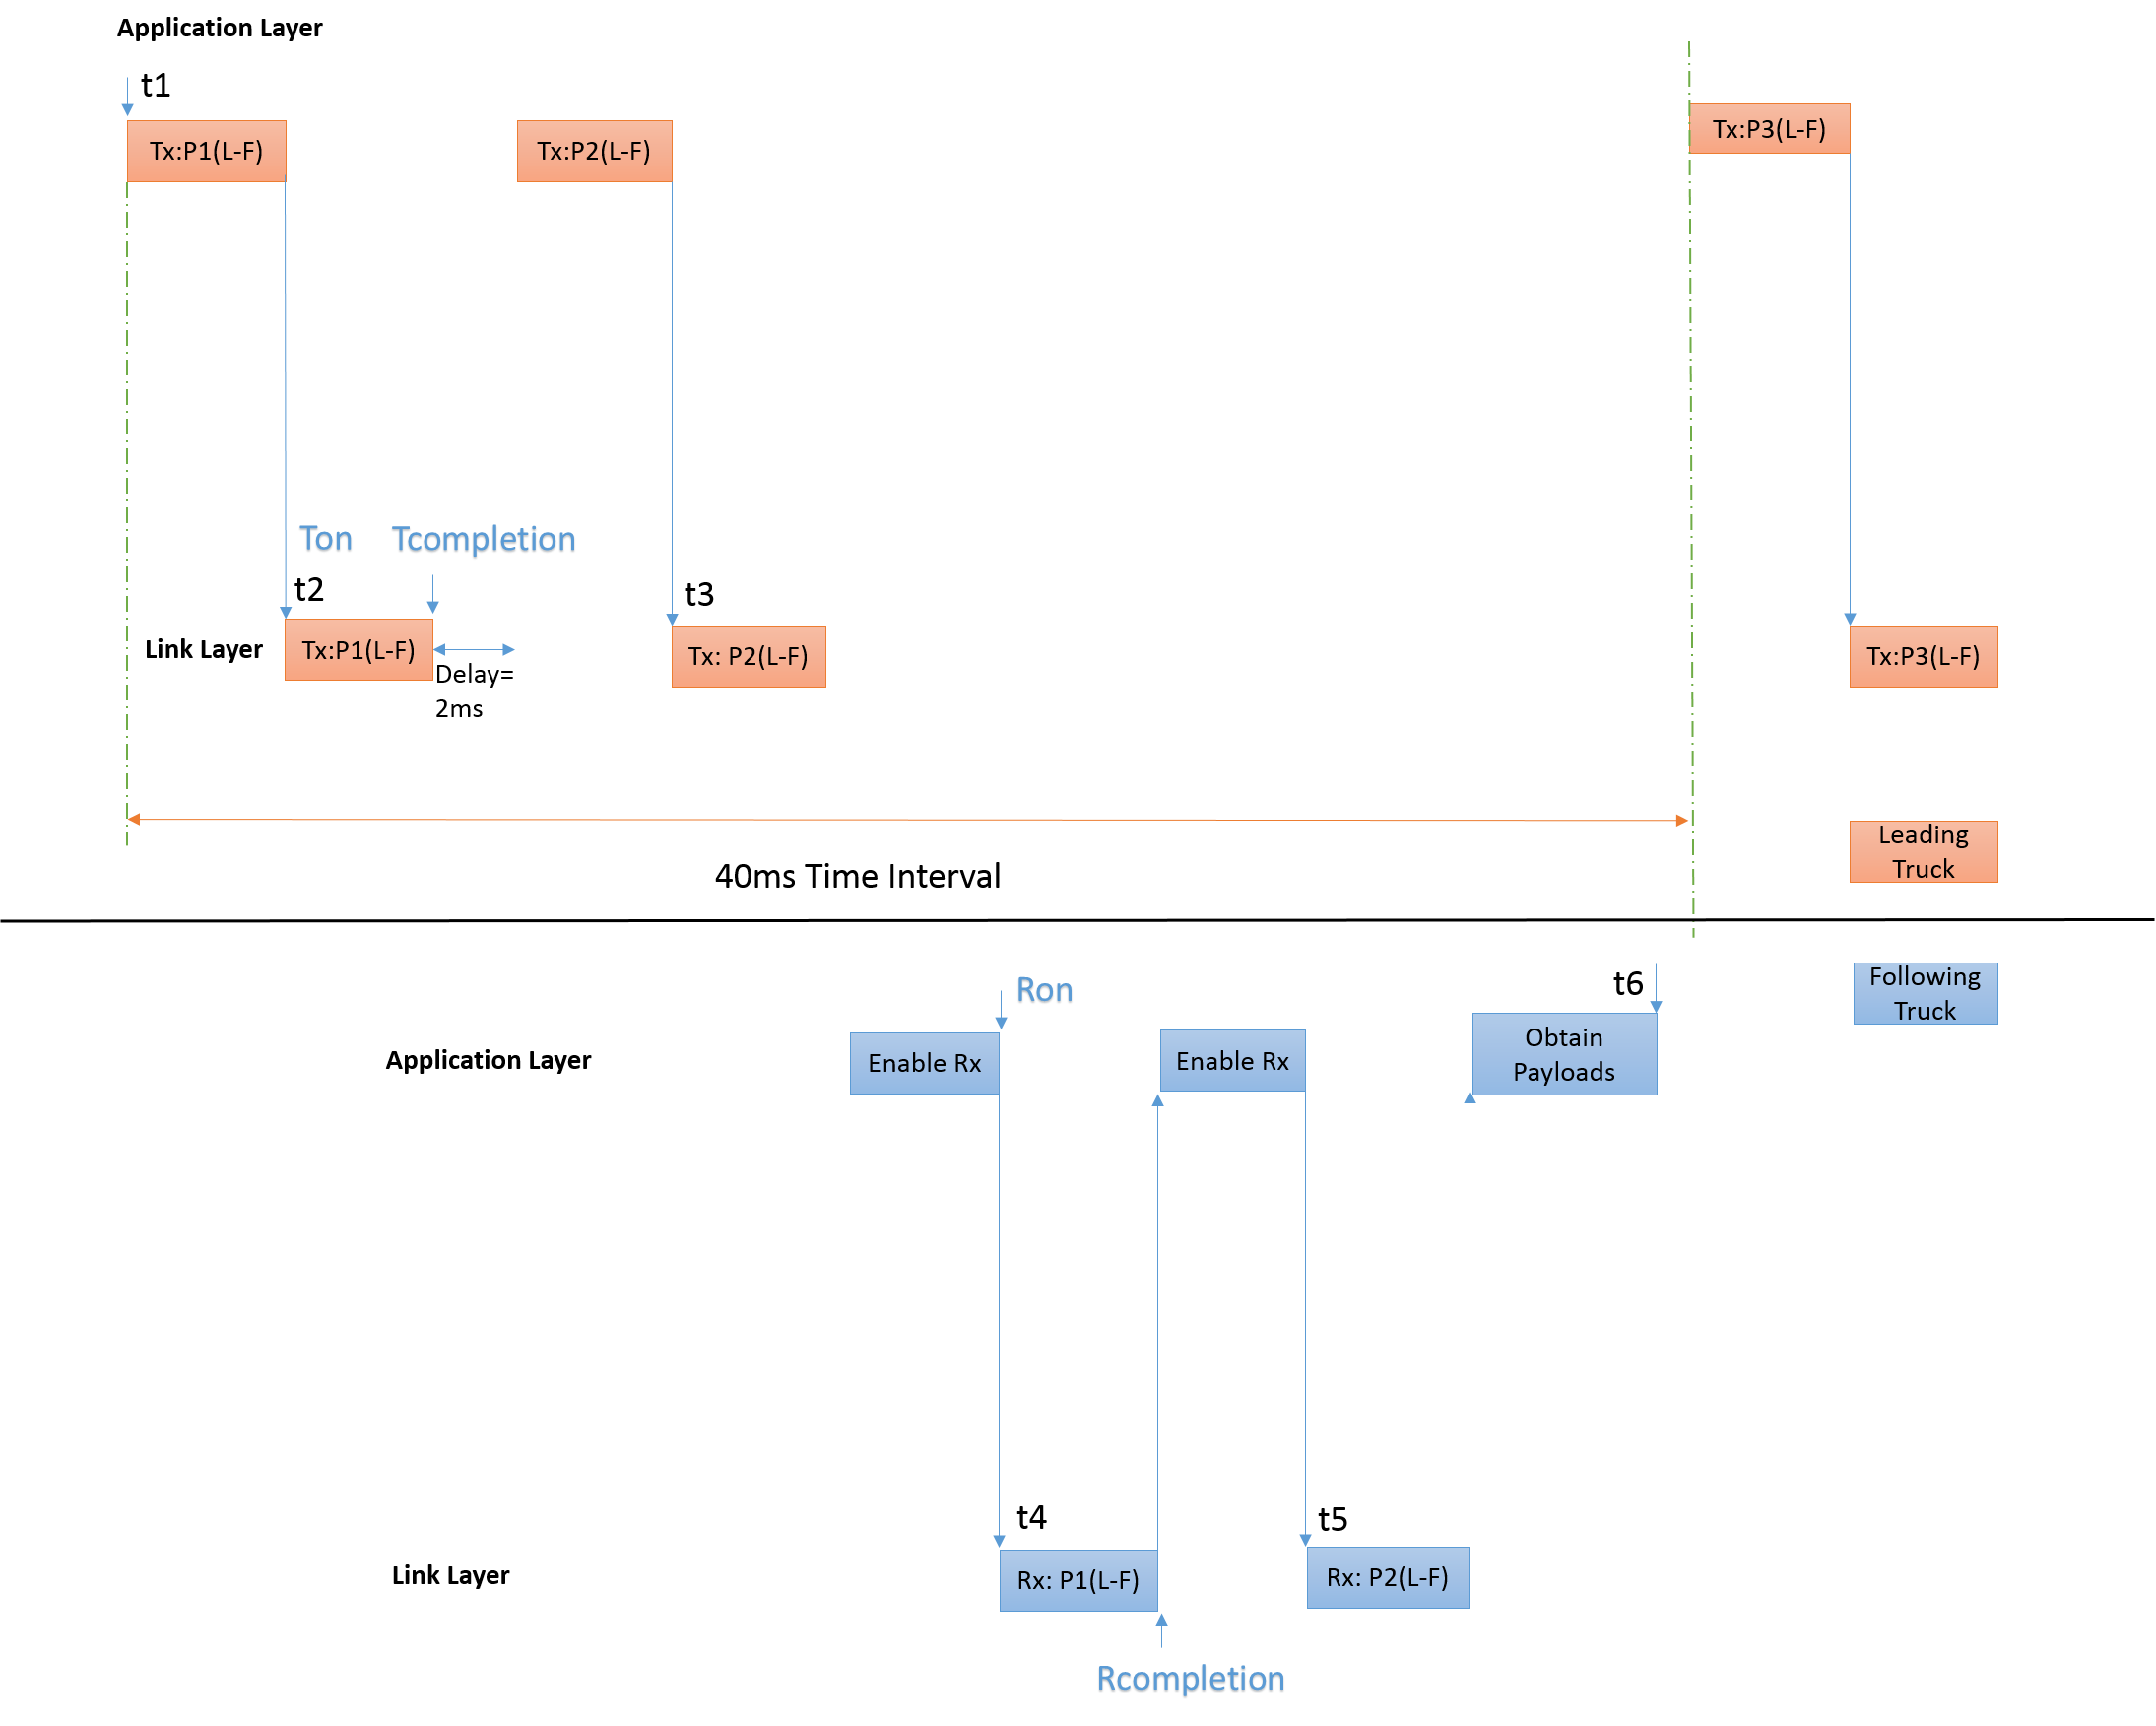
\includegraphics[width=1\textwidth]{figures/IndicationofLoggingParameters}
    \centering
    \caption{Logged parameters to determine appropriate working of the system}
    \label{fig:LoggedParametersDetermineAppWorking}    
\end{figure}




\subsection{MATLAB Implementation}
To process large data files created in the format as shown in Listing \ref{lst:loggingFormat}, we handle the log specific to each configuration at a time, on processing the log unique to that configuration completely; we go ahead with processing the log unique to the following configuration. Following this approach helps us to avoid storing significant amounts of data in memory which could lead to a MATLAB crash. On processing all the logs, we store the information appropriately so as to create desired graphs such as PER vs. Channel, MER vs. Channel, PER vs. Distance, Measured Distance vs. Calculated Distance, etc.

The parsing is implemented by obtaining the lines containing the string "messageLatency" from the log and stored in a cell array. A single row is created for each message with columns representing the parameter and its corresponding values. Depending on the number of messages and packets per message tested, appropriate number of lines are read that are specific to each configuration. The parameters packets per message, the number of messages, actual measured distance and the number of configurations tested and paths to the log files need to be input before running the post processing script.

The obtained cell array after parsing the log files is used for further processing. Based on the required results like PER, MER, message latency, packet latency, the accuracy of ranging, etc. the obtained cell array is traversed for the desired parameters and after applying the desired modifications on the data, it is stored in separate arrays corresponding to each result. Each row in these separate arrays corresponds to an average of all the values for the desired parameter in that specific configuration, and the column in these separate arrays corresponds to each run. It is to be noted that the cell array obtained by parsing the log files needs to be converted to numbers from strings to process them as indicated above. This process continues for all the configurations across all runs.

From these separate arrays, we obtain data and classify them based on channel, data rate, Preamble length, etc. by correlating with the configuration number. Consequently, the data is further processed based on the required result and the classification, and corresponding graphs created. The MATLAB implementation is such that it can process logs for up to four packets per message and any desired number of configurations and runs.

It is to be noted that based on the configurations that are tested, the code for classification needs to be modified because classification is performed by correlating with the configuration number. The MATLAB implementation currently calculates PER at leading truck, PER at following truck, MER at leading truck, MER at following truck, packet latency for leading truck (mean, min, max and standard deviation), packet latency for following truck (mean, min, max and standard deviation), message latency in leading truck (mean, min, max and standard deviation), message latency in following truck (mean, min, max and standard deviation), range accuracy, RX level at leading truck for each packet of a message (mean, min, max and standard deviation) and RX level at following truck for each packet of a message (mean, min, max and standard deviation). The MATLAB implementation allows creation of graphs with respect to the parameters stated above.